%\documentclass[11pt,letterpaper]{article}
\documentclass[oneside,11pt]{amsart}

%\usepackage{a4wide}
%\usepackage{epsfig}
%\usepackage{psfig}
\usepackage{graphicx}
\usepackage{natbib,latexsym,url,enumitem,pdfpages}
\usepackage{color}
\usepackage{wrapfig}
\usepackage{caption}

\captionsetup{
    justification=justified,
    margin=0pt,
    font=small}

% Some fancy commenting
\definecolor{todo}{RGB}{200,0,0}
\newcommand{\comment}[2][todo]{{\color{#1}[[{\bf #2}]]}}

% Challenge counter
\newcounter{chalno}
\newcommand{\chal}[1]{\refstepcounter{chalno}\label{#1}}

% User commands
\makeatletter
\let\jnl@style=\rm
\def\ref@jnl#1{{\jnl@style#1}}

\def\ref@jnl#1{{\jnl@style#1}}% 
\newcommand\aj{\ref@jnl{AJ}}%        % Astronomical Journal 
\newcommand\araa{\ref@jnl{ARA\&A}}%  % Annual Review of Astron and Astrophys 
\newcommand\apj{\ref@jnl{ApJ}}%    % Astrophysical Journal ++
\newcommand\apjl{\ref@jnl{ApJL}}     % Astrophysical Journal, Letters 
\newcommand\apjs{\ref@jnl{ApJS}}%    % Astrophysical Journal, Supplement 
\newcommand\ao{\ref@jnl{ApOpt}}%   % Applied Optics ++
\newcommand\apss{\ref@jnl{Ap\&SS}}%  % Astrophysics and Space Science 
\newcommand\aap{\ref@jnl{A\&A}}%     % Astronomy and Astrophysics 
\newcommand\aapr{\ref@jnl{A\&A~Rv}}%  % Astronomy and Astrophysics Reviews 
\newcommand\aaps{\ref@jnl{A\&AS}}%    % Astronomy and Astrophysics, Supplement 
\newcommand\azh{\ref@jnl{AZh}}%       % Astronomicheskii Zhurnal 
\newcommand\baas{\ref@jnl{BAAS}}%     % Bulletin of the AAS 
\newcommand\icarus{\ref@jnl{Icarus}}% % Icarus
\newcommand\jrasc{\ref@jnl{JRASC}}%   % Journal of the RAS of Canada 
\newcommand\memras{\ref@jnl{MmRAS}}%  % Memoirs of the RAS 
\newcommand\mnras{\ref@jnl{MNRAS}}%   % Monthly Notices of the RAS 
\newcommand\pra{\ref@jnl{PhRvA}}% % Physical Review A: General Physics ++
\newcommand\prb{\ref@jnl{PhRvB}}% % Physical Review B: Solid State ++
\newcommand\prc{\ref@jnl{PhRvC}}% % Physical Review C ++
\newcommand\prd{\ref@jnl{PhRvD}}% % Physical Review D ++
\newcommand\pre{\ref@jnl{PhRvE}}% % Physical Review E ++
\newcommand\prl{\ref@jnl{PhRvL}}% % Physical Review Letters 
\newcommand\pasp{\ref@jnl{PASP}}%     % Publications of the ASP 
\newcommand\pasj{\ref@jnl{PASJ}}%     % Publications of the ASJ 
\newcommand\qjras{\ref@jnl{QJRAS}}%   % Quarterly Journal of the RAS 
\newcommand\skytel{\ref@jnl{S\&T}}%   % Sky and Telescope 
\newcommand\solphys{\ref@jnl{SoPh}}% % Solar Physics 
\newcommand\sovast{\ref@jnl{Soviet~Ast.}}% % Soviet Astronomy 
\newcommand\ssr{\ref@jnl{SSRv}}% % Space Science Reviews 
\newcommand\zap{\ref@jnl{ZA}}%       % Zeitschrift fuer Astrophysik 
\newcommand\nat{\ref@jnl{Nature}}%  % Nature 
\newcommand\iaucirc{\ref@jnl{IAUC}}% % IAU Cirulars 
\newcommand\aplett{\ref@jnl{Astrophys.~Lett.}}%  % Astrophysics Letters 
\newcommand\apspr{\ref@jnl{Astrophys.~Space~Phys.~Res.}}% % Astrophysics Space Physics Research 
\newcommand\bain{\ref@jnl{BAN}}% % Bulletin Astronomical Institute of the Netherlands 
\newcommand\fcp{\ref@jnl{FCPh}}%   % Fundamental Cosmic Physics 
\newcommand\gca{\ref@jnl{GeoCoA}}% % Geochimica Cosmochimica Acta 
\newcommand\grl{\ref@jnl{Geophys.~Res.~Lett.}}%  % Geophysics Research Letters 
\newcommand\jcp{\ref@jnl{JChPh}}%     % Journal of Chemical Physics 
\newcommand\jgr{\ref@jnl{J.~Geophys.~Res.}}%     % Journal of Geophysics Research 
\newcommand\jqsrt{\ref@jnl{JQSRT}}%   % Journal of Quantitiative Spectroscopy and Radiative Trasfer 
\newcommand\memsai{\ref@jnl{MmSAI}}% % Mem. Societa Astronomica Italiana 
\newcommand\nphysa{\ref@jnl{NuPhA}}%     % Nuclear Physics A 
\newcommand\physrep{\ref@jnl{PhR}}%       % Physics Reports 
\newcommand\physscr{\ref@jnl{PhyS}}%        % Physica Scripta 
\newcommand\planss{\ref@jnl{Planet.~Space~Sci.}}%  % Planetary Space Science 
\newcommand\procspie{\ref@jnl{Proc.~SPIE}}%      % Proceedings of the SPIE 

\newcommand\actaa{\ref@jnl{AcA}}%  % Acta Astronomica
\newcommand\caa{\ref@jnl{ChA\&A}}%  % Chinese Astronomy and Astrophysics
\newcommand\cjaa{\ref@jnl{ChJA\&A}}%  % Chinese Journal of Astronomy and Astrophysics
\newcommand\jcap{\ref@jnl{JCAP}}%  % Journal of Cosmology and Astroparticle Physics
\newcommand\na{\ref@jnl{NewA}}%  % New Astronomy
\newcommand\nar{\ref@jnl{NewAR}}%  % New Astronomy Review
\newcommand\pasa{\ref@jnl{PASA}}%  % Publications of the Astron. Soc. of Australia
\newcommand\rmxaa{\ref@jnl{RMxAA}}%  % Revista Mexicana de Astronomia y Astrofisica

%% added feb 9, 2016
\newcommand\maps{\ref@jnl{M\&PS}}% Meteoritics and Planetary Science
\newcommand\aas{\ref@jnl{AAS Meeting Abstracts}}% American Astronomical Society Meeting Abstracts
\newcommand\dps{\ref@jnl{AAS/DPS Meeting Abstracts}}% American Astronomical Society/Division for Planetary Sciences Meeting Abstracts



\let\astap=\aap 
\let\apjlett=\apjl 
\let\apjsupp=\apjs 
\let\applopt=\ao 



\DeclareRobustCommand{\gtrsim}{%
\mathrel{\hskip-.5em\begin{array}{c}>\\[-8pt]\sim\end{array}\hskip-.5em}}
\DeclareRobustCommand{\lesssim}{%
\mathrel{\hskip-.5em\begin{array}{c}<\\[-8pt]\sim\end{array}\hskip-.5em}}

\pretolerance=10000
\textwidth=6.4in
\textheight=8.95in
\voffset = 0.in
%\voffset = -0.3in  % For my printer
\topmargin=0.0in
\headheight=0.00in
\hoffset = 0.0in
%\hoffset = 0.33in  %  For my printer
\headsep=0.00in
\oddsidemargin=0in
\evensidemargin=0in
\parindent=2em
\parskip=0.2ex
 
\renewcommand{\baselinestretch}{1.03}

\special{papersize=8.5in,11in}

\newcommand{\markus}{\textcolor{green}}
\newcommand{\request}{\$376k}

\setlength{\parskip}{0.6 ex plus 0.4ex minus 0.2ex} \flushbottom
\pagestyle{plain} 

% From the call:
%
% For Phase A system design proposals, the project description should
% be no more than 10 pages devoted to science cases, conceptual
% designs, and a preliminary budget and schedule for the full build of
% the instrument. Up to two additional pages are allowed for the Phase
% A system design budget, milestones, deliverables, and references for
% the proposed work. For both proposal types, the requested budget
% should be in summary form identifying how the money will be spent on
% major study costs. To gain an initial understanding of technical
% issues such as existing instrument configurations, observatory
% interfaces, and guidelines for the standard WMKO instrument
% development process, proposers are strongly encouraged to contact the
% WMKO Instrument Program Manager, Marc Kassis.

\begin{document}
% \thispagestyle{empty}

\pagenumbering{arabic}

\vspace*{-1.5cm}

\centerline{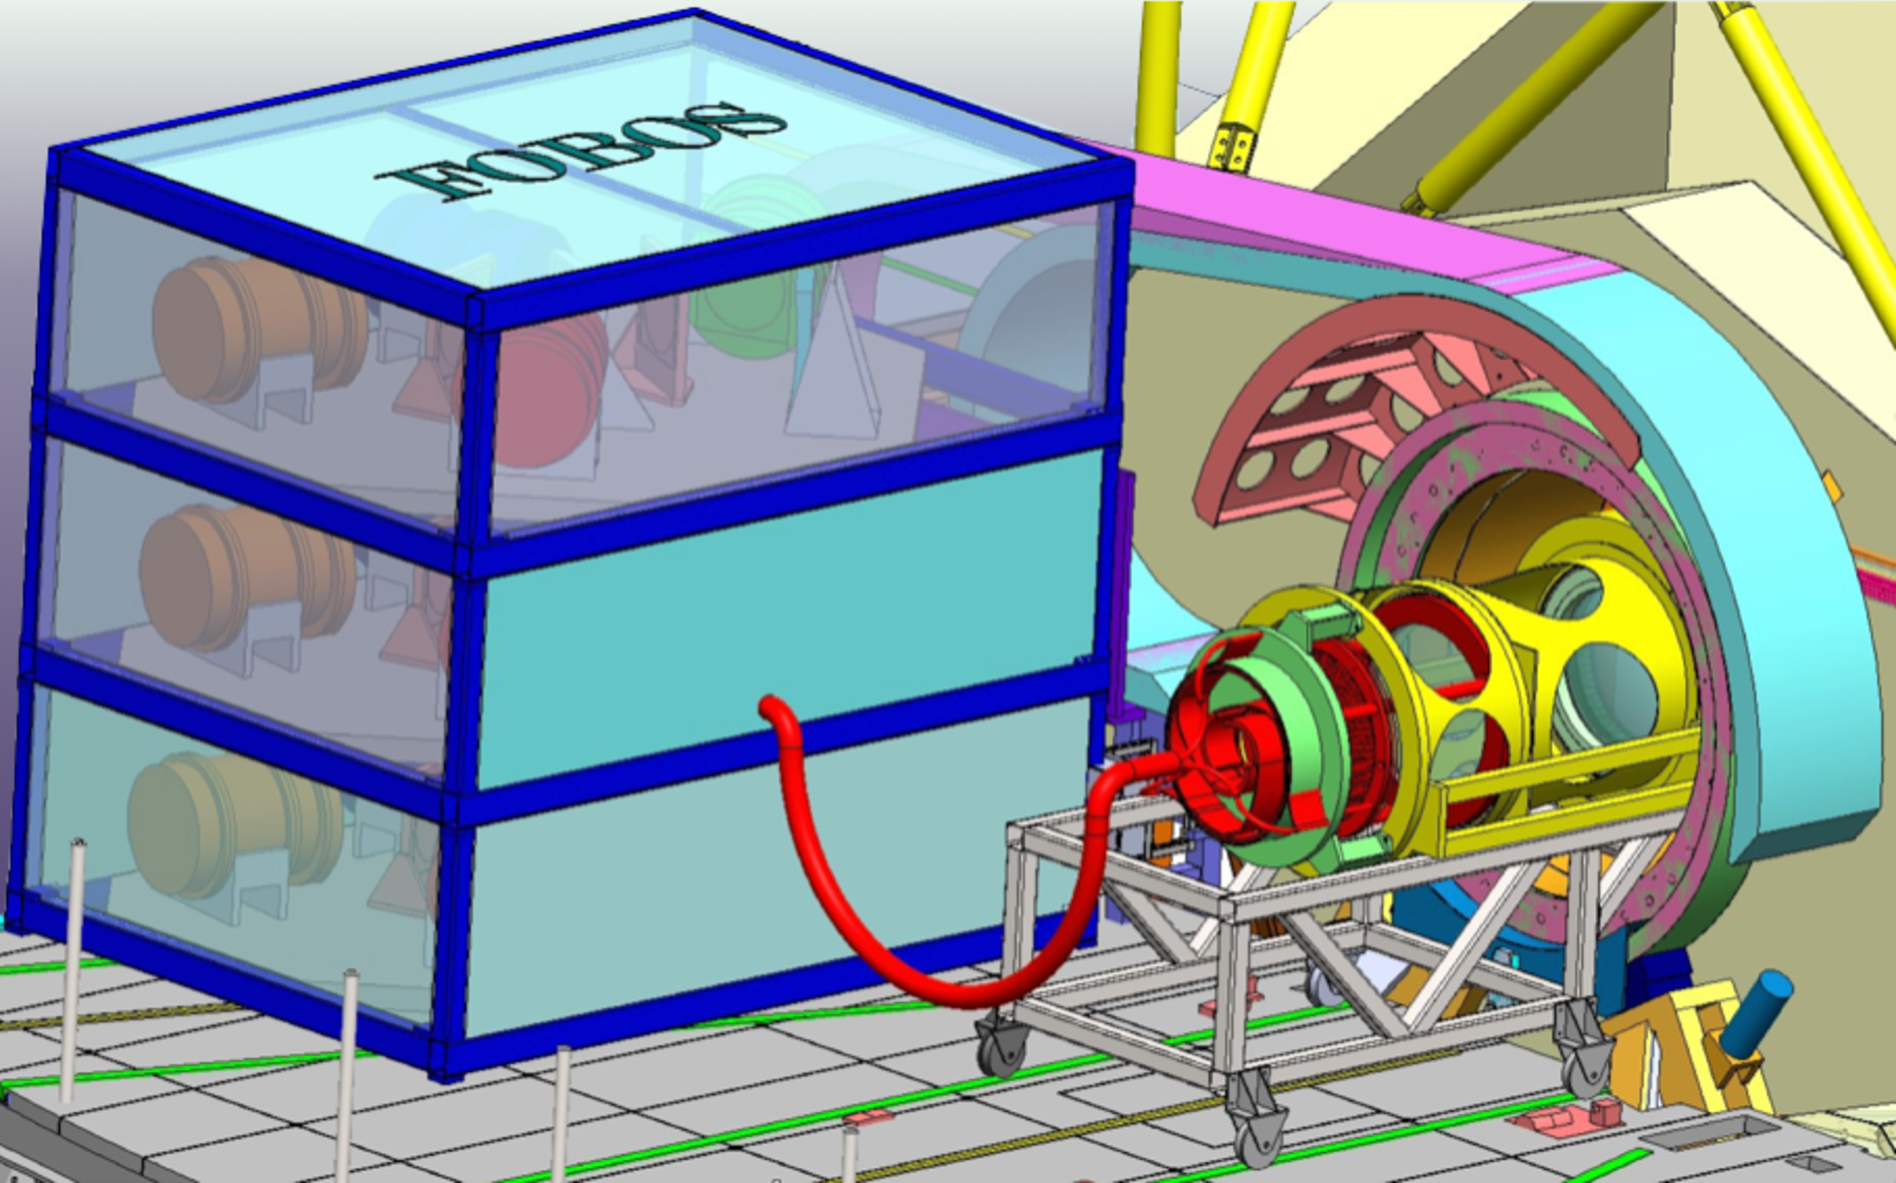
\includegraphics[width=0.5\textwidth]{figs/FOBOS_inst_v2.pdf}}
\centerline{\textsc {\Large FOBOS: The Fiber-Optic Broadband Optical Spectrograph}}
\smallskip
\centerline{\large\it Keck's next-generation spectroscopic facility}

%% Executive Summary and Overview
%%%%
% -- Overview Material
% --     FOBOS Keck White Paper 2019
%%%%

%\setcounter{secnumdepth}{0}
\section*{Executive Summary}
%\setcounter{secnumdepth}{1}

% Soon, our community will be inundated with sources of interest from
% large-scale ground- and space-based surveys requiring spectroscopic
% follow-up for physical characterization. In fact, with the recent
% {\it Gaia} releases, the spectroscopic needs in Galactic Astronomy
% are already dire, a situation that will be acutely felt by
% extragalactic community once LSST, Euclid, and WFIRST begin
% delivering data. These sources will span the full range of scientific
% interests of our current Keck partners and Keck's current
% spectroscopic capabilities will not e sufficient to meet these needs.

The 2016 Keck Observatory Scientific Strategic Plan lists
highly-multiplexed spectroscopy as a key desirable that would
position Keck to take advantage of the coming era of wide-field
imaging facilities like LSST, Euclid, and WFIRST. FOBOS addresses
this priority via a fiber-based facility that optimizes depth over
area, preserving Keck's historical strength in faint-object
spectroscopy. The result is a uniquely blue-sensitive, high-multiplex
instrument with order-of-magnitude greater sampling density than
competitors like Subaru's Prime Focus Spectrograph (PFS). In the LSST
era, FOBOS will excel at building the deep, spectroscopic reference
data sets needed to interpret vast imaging data. At the same time,
its flexible focal plane, including deployable integral-field units
(IFUs), enables an expansive range of scientific investigations from
the diverse Keck community.

FOBOS is a modular instrument composed of three major components: (1)
an atmospheric dispersion corrector (ADC) whose final lens traces the
Nasmyth focal surface, (2) a flexible focal-plane sampling system
that deploys as many as 1800 free-roaming Starbug positioners that
``walk'' on this surface to sample a 17-arcminute diameter field, and
(3) a bank of three temperature-controlled bench spectrographs
mounted on the Nasmyth platform that provide $R \sim 3500$
spectroscopy over an instantaneous bandpass of 0.31-1$\mu$m. The
spectrographs are fed light from the focal plane by a short fiber run
($<$10 m) through a stress-relief cabling system to minimize
throughput losses (see diagram above).

The focal-plane system is designed to allow for flexible targeting
and multiple sampling formats. When configured in its single-fiber
mode, each Starbug carries a single optical fiber with a 150 $\mu$m
diameter core fed by demagnifying fore-optics that sample a
0.9-arcsec diameter on-sky aperture. When configured in multi-IFU
mode, FOBOS deploys a different suite of Starbugs carrying fiber
bundles with coupled lenslet arrays that provide finer spatial
sampling.  Its flexible focal
plane allows efficient observing strategies that combine multiple
programs and can dynamically respond to changing conditions and
targets of opportunity.

% Finally, a monolithic-IFU mode provides uniform coverage
% over a $\gtrsim$0.5 arcmin$^2$ field-of-view.

Its UV sensitivity, high multiplex and sampling density, multiple
focal-plane sampling options, and flexible targeting system make
FOBOS compelling in science areas that are both traditional strengths
of the Keck Community and unique among the capabilities of
forthcoming spectroscopic facilities. Science cases discussed in
Section \ref{sec:goals} include: Local Group archeology via resolved
stellar spectra in dwarf galaxies, M31, and the Milky Way halo;
globular-cluster populations of individual galaxies and Coma-like
galaxy clusters; new probes of galaxies, their environments, and the
evolution of both since $z \sim 1$ including kinematic studies of
winds, resolved gas-phase properties and dynamics of star-forming
galaxies, and the internal structure of stellar populations for large
samples of distant galaxies; detailed tomographic Ly-$\alpha$ and
UV-absorption-line measurements of galaxies and the intergalactic
medium at $z \sim 2$--4; direct, spectroscopy redshifts critical to
the success of cosmological analyses based on photo-$z$ measurements
from panoramic deep imaging (e.g., LSST); and rapid follow-up of
transient sources with a dedicated fixed IFU at the field center.

This Keck White Paper proposal requests Phase-A funding to complete conceptual design, develop cost estimates, plan for upcoming NSF and other funding opportunities, and advance solutions to high-risk design elements.  

% FOBOS enables Local Group archeology studies via resolved stellar
% spectra at moderate spectral resolution in dwarf galaxies, M31, and
% the Milky Way halo. At greater distances, FOBOS will compile powerful
% statistics for the globular-cluster populations of individual
% galaxies and Coma-like galaxy clusters. FOBOS's combined depth and
% high sampling density allow for new probes of galaxies, their
% environments, and a their mutual evolution from $z \sim 1$.
% Specifically when using its IFU mode, FOBOS will enable kinematic
% studies of winds, the resolved gas-phase properties and dynamics of
% star-forming galaxies, and the internal structure of stellar
% populations for large samples of distant galaxies. FOBOS's capacity
% for detailed tomographic Ly-$\alpha$ and UV-absorption-line
% measurements of galaxies and the intergalactic medium at $z \sim
% 2$--4 will be unparalleled. Cosmological analyses using panoramic
% deep imaging (e.g., LSST) will greatly benefit from photo-$z$
% training by FOBOS, which is ideally suited to required photo-$z$
% programs. Finally, with a dedicated IFU always ready, FOBOS can
% rapidly follow up transient sources while continuing to collect
% valuable photons on background targets.



% High-multiplex and deep spectroscopic followup of LSST and other
% panoramic deep-imaging surveys is a widely recognized necessity.
% Reports in 2015 and 2016 by the National Research Council and
% National Optical Astronomical Observatory specifically recommended
% investment in new spectroscopic facilities to meet these needs
% because none currently exist or are planned for U.S.\ observatories.
% We seek seed funding from WMKO to continue conceptual design of
% FOBOS, a powerful new spectrograph for the Keck II telescope that increases its current survey speed by a factor of X.

% Led by NSF's Large Synoptic Survey Telescope\footnote{
% %
% LSST will be begin science operations in 2023.}
% %
% (LSST), astronomy is entering a new era of unprecedented deep-imaging data sets that will survey huge volumes of the
% Universe.  From the emergence of the earliest galaxies from a ``primordial soup'' of gas and dust, to the peak of
% cosmic star formation and the current era of accelerated expansion, these surveys will provide unprecedented statistics
% at key epochs of cosmic history.


% Even so, gaining physical insight from panoramic imaging surveys will require intensive spectroscopic follow-up.  The
% power of combining photometry and dedicated spectroscopy is widely appreciated and perhaps best illustrated by the
% success of the Sloan Digital Sky Survey (SDSS) which used this combination to record the properties of over 1 million
% galaxies, mapping the present-day universe and making SDSS one of the most highly cited surveys in the history of
% astronomy.

% LSST's all-sky images will be 1,000 times deeper and detect far more
% distant galaxies than SDSS, but \textbf{no current U.S. facility is
% capable of obtaining spectroscopic follow-up of LSST galaxies} at a level
% required to capitalize on the \$1B the U.S.\ has invested in that
% project.  In fact, an SDSS-like spectroscopic study of 1 million
% galaxies at LSST depth would require 300 years of observing on the
% largest telescopes with current instrumentation!  

% Solving this problem requires not only more powerful spectroscopic facilities, but new ways to take better advantage of
% what will be necessarily more limited spectroscopy compared to the vast imaging surveys of the LSST era.  The more
% promising path is encapsulated in one of NSF's ``10 Big Ideas,'' \emph{Harnessing the Data Revolution}: we can maximize
% the information content of LSST and other imaging facilities via machine learning from optimally designed spectroscopic
% training sets.


% The need for spectroscopic follow-up in the LSST era was made clear in
% the National Research Council's 2015 report, ``Optimizing the U.S.
% Ground-Based Optical and Infrared Astronomy System'' \citep{NAP21722}:
% %
% \noindent\begin{center}\mbox{\parbox{0.95\linewidth}{
% %
% The National Science Foundation should support the development of a
% wide-field, highly multiplexed spectroscopic capability on a medium- or
% large-aperture telescope in the Southern Hemisphere to enable a wide
% variety of science, including follow-up spectroscopy of Large Synoptic
% Survey Telescope targets. Examples of enabled science are studies of
% cosmology, galaxy evolution, quasars, and the Milky Way.
% %
% }}\end{center}

% Workshops organized by the National Optical Astronomy Observatory (NOAO)
% in 2013 and 2016, the latter at the NSF's request, reported specific
% spectroscopic needs for LSST follow-up in all science areas.  In
% particular, the 2016 report notes that a critical resource in need of
% prompt development is to ``Develop or obtain access to a highly
% multiplexed, wide-field optical multi-object spectroscopic capability on
% an 8m-class telescope.''  Based on these recommendations, we propose the
% FOBOS instrument coupled with a suite of data-driven tools to address
% the spectroscopic requirements of LSST and other photometric surveys at
% a final cost 20 times less than a new Southern Hemisphere facility.
% Located in Hawaii, FOBOS can access more than 70\% of the LSST
% footprint, more than adequate for building powerful
% spectroscopic training sets.  Compared to the Prime Focus Spectrograph
% (PFS) on Japan's Subaru Telescope, FOBOS would be 1.7$\times$ faster,
% provide unique UV sensitivity (0.31--1 $\mu$m compared to
% 0.38--1.25 $\mu$m with PFS), and offer higher-density, more flexible
% target sampling over ``deep-drilling'' fields.  Unlike PFS, FOBOS would be operated
% on a U.S.\ telescope with dedicated U.S.\ access and a commitment to
% supporting U.S.-led imaging facilities.  FOBOS is also complementary to
% future telescopes and instruments that would be optimized to cover wider areas
% (several deg$^2$ per pointing) at shallower depths.

%\comment{mention FOBOS can do PI-led science too}

% The need for deep spectroscopic follow-up is particularly acute for the major cosmological probes to be carried out by
% LSST, Euclid, and WFIRST, which all rely on ``photometric redshifts:'' measures of galaxy redshift, $z$
% --- a direct proxy of distance and look-back time---based on imaging alone. \citet{newman15} summarize the case for a
%     significant spectroscopic campaign to calibrate and train LSST photometric redshifts in order to improve cosmological constraints.  They describe a redshift survey that,
%     if carried out with FOBOS, would increase LSST's Dark Energy figure-of-merit by 40\% at a cost of less than 5\% of
%     the LSST budget.  The urgent case for spectroscopic redshift training has been the subject of numerous publications
%     \citep[e.g.,][]{laureijs11, masters15, hemmati18}.

% Meanwhile, the astronomy community recognizes that the coming ``Big
% Data'' era, culminating in LSST, necessitates ``\textbf{harnessing the
% data revolution}.''  Widespread community interest in advanced
% data-science techniques continues to grow amidst calls for educational
% programs, conference series, and research funding to support the growth
% of a new field, ``Astroinformatics,'' which exploits the interface
% between astrophysics and statistics \citep{borne09}.  Astronomy's
% largest organizations, including the American Astronomical Society and
% the International Astronomical Union, have supported active working
% groups on astroinformatics and astrostatistics since 2015.  LSST itself
% has supported the Informatics and Statistics Science Collaboration and
% partnered with NSF on the Data Science Fellowship Program to train
% astronomy graduate students in data-science techniques.  Our proposal
% builds on and contributes to these ongoing efforts.



\section{Science Drivers}
\label{sec:goals}

\comment{this needs some reorganization}

%-----------------------------------------------------------------------
%%%%
% -- Local Group Science Cases
% --     FOBOS Keck White Paper 2019
%%%%

\subsection{Resolved studies of Local Group galaxies}
%Unraveling the Formation History of our Local Group of Galaxies}
\label{sec:localgroup}

By resolving their constituent parts, galaxies in our Local Group
(LG) --- the Milky Way (MW), the Magellanic Clouds, Andromeda (M31),
Triangulum (M33), and numerous satellite galaxies
--- provide a unique perspective on the evolution of galaxies and
large-scale structure. In particular, the remnants of the
hierarchical merging process are revealed by the population of LG
dwarf galaxies and other stellar substructures in the halos of the MW
and M31. In the coming decade, imaging data from LSST and WFIRST will
increase the census of stellar streams and halo substructure in both
the Milky Way and Andromeda by a hundredfold. FOBOS spectroscopy of
these structures will, e.g., constrain stream orbits and the total
mass they enclose \citep{2017ApJ...836..234S}. These data will also
provide age and chemical composition measurements either directly or
via targeted machine-learning applications \citep[see Section
\ref{sec:datascience};][]{2015ApJ...808...16N, 2018arXiv180401530T,
2018arXiv180803278T}. FOBOS is well-suited to these observations by
dramatically improving the survey speed over DEIMOS (by an order of
mangitude or more) and will remain sensitive enough to push toward
the main-sequence turn-off of MW substructures. Compared to the MW,
studies of M31's disk and halo are more suited for dedicated FOBOS
programs. Indeed, the dramatic improvement in survey speed will,
e.g., yield a direct measurements of secular processes active in
M31's disk, such as radial migration and vertical disk heating
\citep{2013ApJ...779..103D, 2015ApJ...803...24D,
2019ApJ...871...11Q}. Even so, {\it Gaia} targets, particularly at
larger distances and higher target densities in the bulge, bar and
inner disk, will prove uniquely suitable for FOBOS spectroscopy.

%\comment{Guhathakurta, Rockosi, Weisz}

% \chal{mwhalo} 
% %
% \item[] {\textsf {\large  Data-Science Challenge \ref{mwhalo}: The
% chemical evolution and assembly history of the MW stellar halo.}}  Using current MW halo models, we will simulate FOBOS
% stellar spectroscopy of main-sequence turn-off
% and red-giant stars in these substructures within the MW that also
% leverages existing data from, e.g., APOGEE and H3.  We will build
% data-driven models based on these data to measure stellar parameters
% (temperature, surface gravity, metallicity, and alpha-element abundance)
% for all halo stars with LSST+2MASS+WISE+WFIRST multi-band photometry,
% allowing us to reconstruct the star-formation history of each disrupted
% satellite. These will be combined with dynamical data and compared with
% cosmological simulations to build a generative model for the assembly
% history of the MW stellar halo.

% \chal{m31} 
% %
% \item[] {\textsf {\large Data-Science Challenge \ref{m31}: The
% differential chemical evolution of M31 and MW.}}  A natural extension of
% Data-Science Challenge \ref{mwhalo} is to perform the same analysis for the
% halo of M31.  However, we cannot expect to obtain high-quality spectra
% of individual main-sequence stars at the distance of M31 with FOBOS.
% Moreover, training a chemical evolution model using spectra of Milky Way
% stars may lead to systematic errors:  The Milky Way and Andromeda have
% distinct evolutionary histories \citep[e.g.][]{2005MNRAS.356.1071R},
% despite being relatively similar in many other respects.  We will
% therefore obtain deep observations of giant stars in the M31 halo to
% drive a machine-learning algorithm that combines a model of the MW halo
% with results from cosmological hydrodynamical simulations to constrain
% the differential history of the MW and M31 stellar halos.

% \chal{gaia} 
% %
% \item[] {\textsf {\large Data-Science Challenge \ref{gaia}: Stellar
% parameter determinations for a billion stellar spectra.}} While
% providing on-sky motions and photometry for 1.7 billion stars in the MW,
% fewer than 10\%, 0.3\%, and 0.1\% of stars will have a full complement
% of astrometrics and kinematics, basic stellar parameters, and chemical
% abundances, respectively.  Moreover, Gaia distance errors increase
% quadratically with distance.  To realize Gaia's full potential, we will
% design FOBOS training sets that, when combined with high-resolution
% datasets from, e.g., APOGEE, WEAVE, will allow us to build data-driven
% models of the absolute magnitude (yielding distance modulus),
% temperature, surface-gravity, and stellar abundance for {\it all} stars
% in the Gaia dataset.  These data will allow us to isolate coeval
% populations in the Galactic disk that can be combined with very
% high-resolution simulations of the Milky Way to provide a detailed
% evolutionary history of our Galactic home.



%%%%
% -- Galaxies Science Cases
% --     FOBOS Keck White Paper 2019
%%%%

\subsection{The dark and luminous content of nearby galaxies}

Using globular cluster and planetary nebulae chemodynamical tracers around nearby galaxies, FOBOS will dramatically
advance dynamical studies of nearby galaxies with $\mathcal{M_\ast/M_\odot} \lesssim 10^{11}$, capturing the majority
of the $\sim$1000 GCs located within $\sim$50 kpc of typical hosts \citep[see][]{2013ApJ...772...82H} and tightly constraining their dark matter halos.  FOBOS's IFU mode will additionally provide powerful insight on the origin of dwarf galaxies, both compact and ultra-diffuse (UDGs), in the field and in nearby clusters like Coma and Virgo.


% which typically host $\lesssim1500$ GCs
% \citep{2013ApJ...772...82H}, FOBOS makes it possible to acquire
% spectra for nearly all GCs located  from the host
% galaxy in a single night. These data will allow us to map the
% chemodynamics of massive galaxy halos and infer orbital families as a
% function of stellar-population properties. Additionally, these data
% will inform models of GC formation in the context of the larger
% galaxy population.

% \subsection{Cluster galaxy populations}

% Presently, it is very expensive to conduct systematic spectroscopic
% studies of the various galaxy types in rich galaxy clusters, like
% Coma, due to their angular spread on the sky. With FOBOS's flexible
% fiber-positioning system and 17-arcminute FOV, it will be possible to
% simultaneously (and efficiently) build up an unprecedented library of
% spectroscopic redshifts and stellar-population parameters of galaxies
% in clusters towards intermediate redshift. Follow-up FOBOS
% observations using its deployable mini-IFUs will allow us to
% simultaneously obtain resolved spectroscopy for 10s of these cluster
% galaxies, enabling us to associate internal structures/properties of
% the galaxies with their host cluster.

\subsection{Internal structure of high-$z$ galaxies}

MaNGA \citep{bundy15} and other large IFU surveys are defining the
$z=0$ benchmark for how internal structure is organized across the
galaxy population. To understand and test ideas for how this internal
structure emerged, we require spatially-resolved observations at $z =
1$--2, just after the peak formation epoch. Indeed, Keck has
pioneered such observations \citep[e.g.,][]{erb04, miller11,law09},
but samples have been limited to a few hundred sources. FOBOS in
multiplex IFU-mode will obtain resolved spectroscopy for thousands of
galaxies. Bright optical emission line tracers will reveal gas-phase
structure and kinematics across unprecedented numbers of early
galaxies. Stacking restframe $\lambda \approx 4500$ spectra will
enable radial stellar population analyses to constrain how stellar
components formed and assembled. While initially limited to coarse
spatial scales, ground-layer adaptive optics (GLAO) in combination with FOBOS would be
transformative for this science. A corrected FWHM of 0.2-0.3 arcsec
would enable fine-sampling IFUs to probe smaller galaxies and study
sub-structure on 1--2 kpc scales.

\subsection{Role of environment at $z=1$--$2$ }

The vast increase in multiplex and high
sampling density will allow FOBOS to map out environmental effects on galaxy evolution at
the group scale ($\mathcal{M_\ast/M_\odot} \lesssim 10^{13}$), and
with sufficient exposure time, for tens of thousands of satellites
down to sub-L$^*$ luminosities. Taking this a step further thanks to
deep, wide-field imaging surveys (e.g., LSST), a 1M-object environmental survey at $z=1$--$2$ may be possible. The
goal is to use improved photo-$z$s, strong priors on spectral types,
and new machine-learning techniques to deliver {\it spectroscopic}
redshifts (with $\lesssim$300 km/s accuracy) at the lowest
signal-to-noise possible, reducing required exposure times by factors of 4--5.

%, 2011AJ....142...72E, 2017AJ....154...28B}

% \noindent\comment{Cooper, further comments?}

% TODO: May be too small...
\begin{wrapfigure}{l}{0.6\textwidth}
%
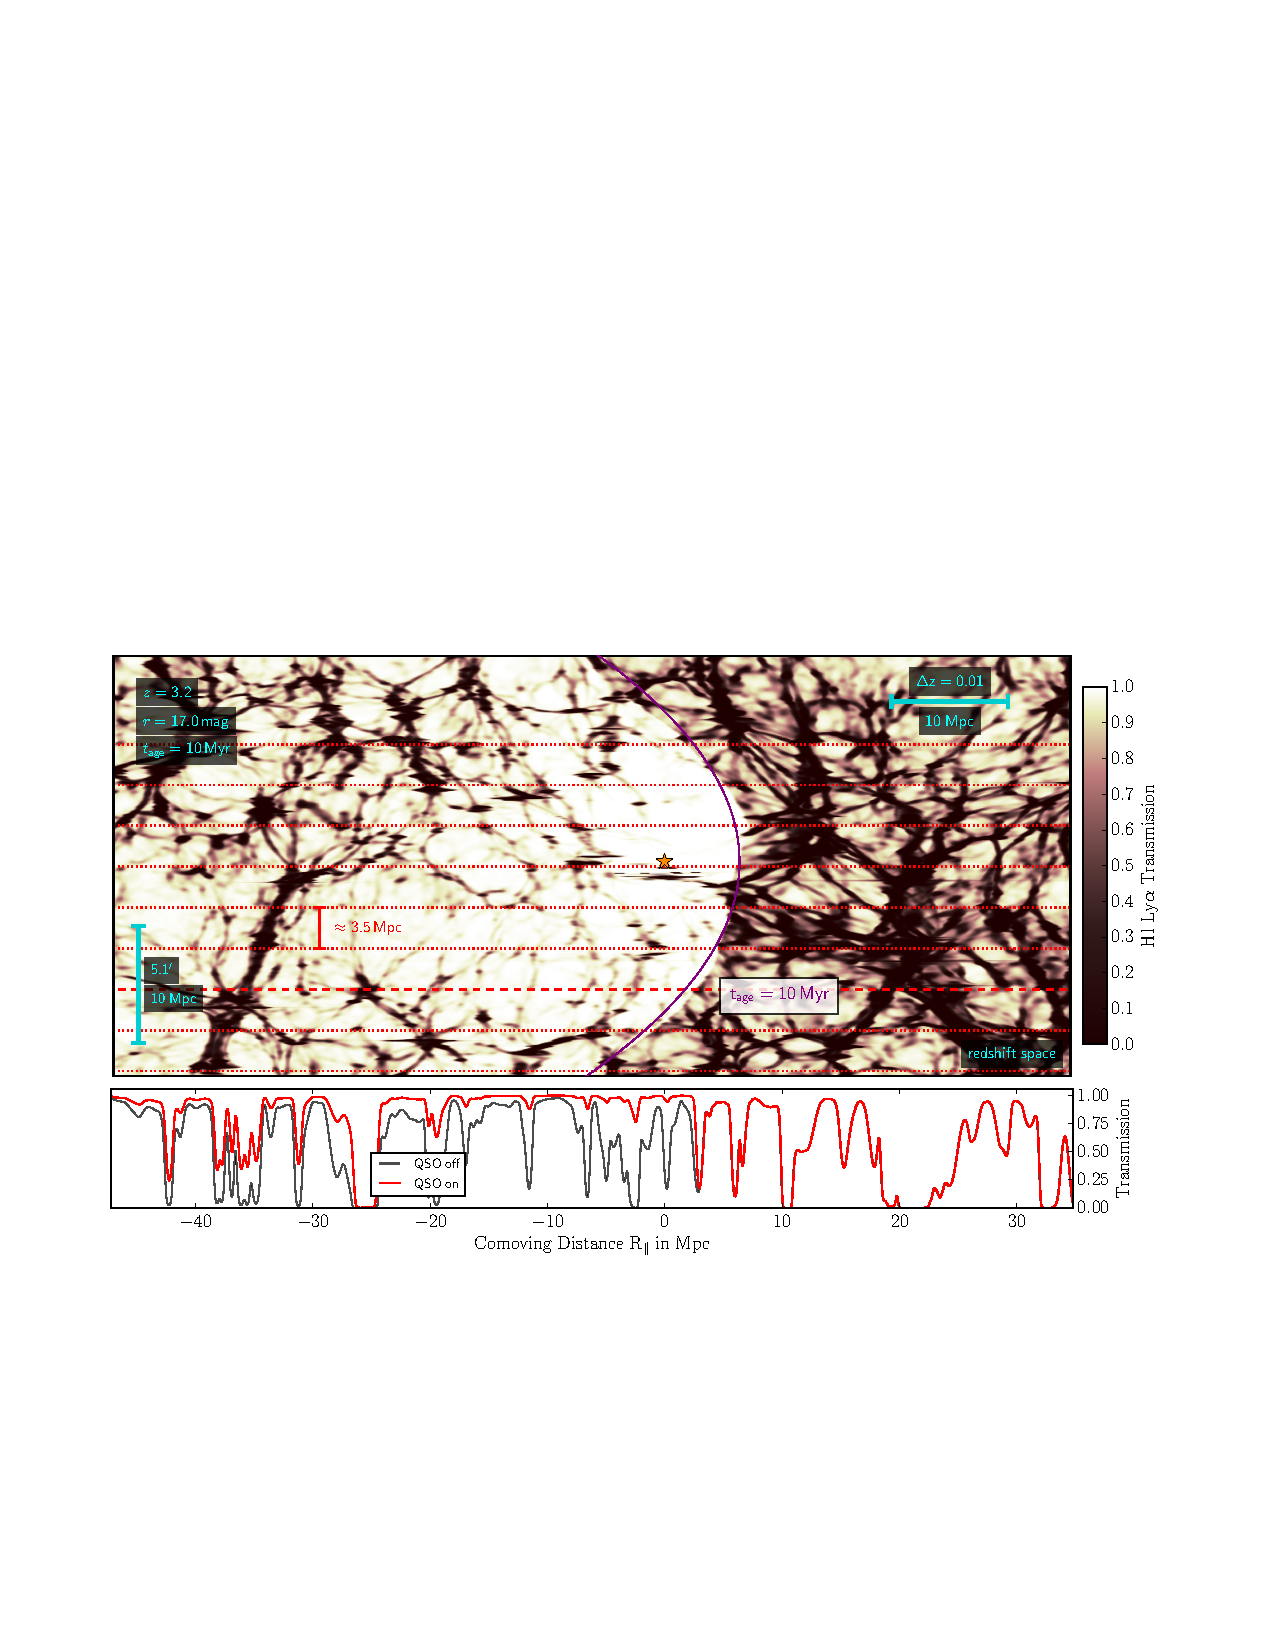
\includegraphics[width=0.6\textwidth]{figs/qso_LightEcho_v1.pdf}
%
\caption{{\it Top}: Quasar ``Light Echos'' revealed in a simulated
tomographic IGM map in the immediate environs of a quasar (gold star)
with several sightlines indicated
\citep[from][]{2018arXiv181005156S}. {\it Bottom}: The ionizing flux
within the echo's extent enhances transmission of Ly$\alpha$ photons
impinging on absorbers along the line-of-sight.}
\label{fig:LightEcho}
\end{wrapfigure}

%\begin{figure}[h!]
%%
%\vskip -0.1in
%%
%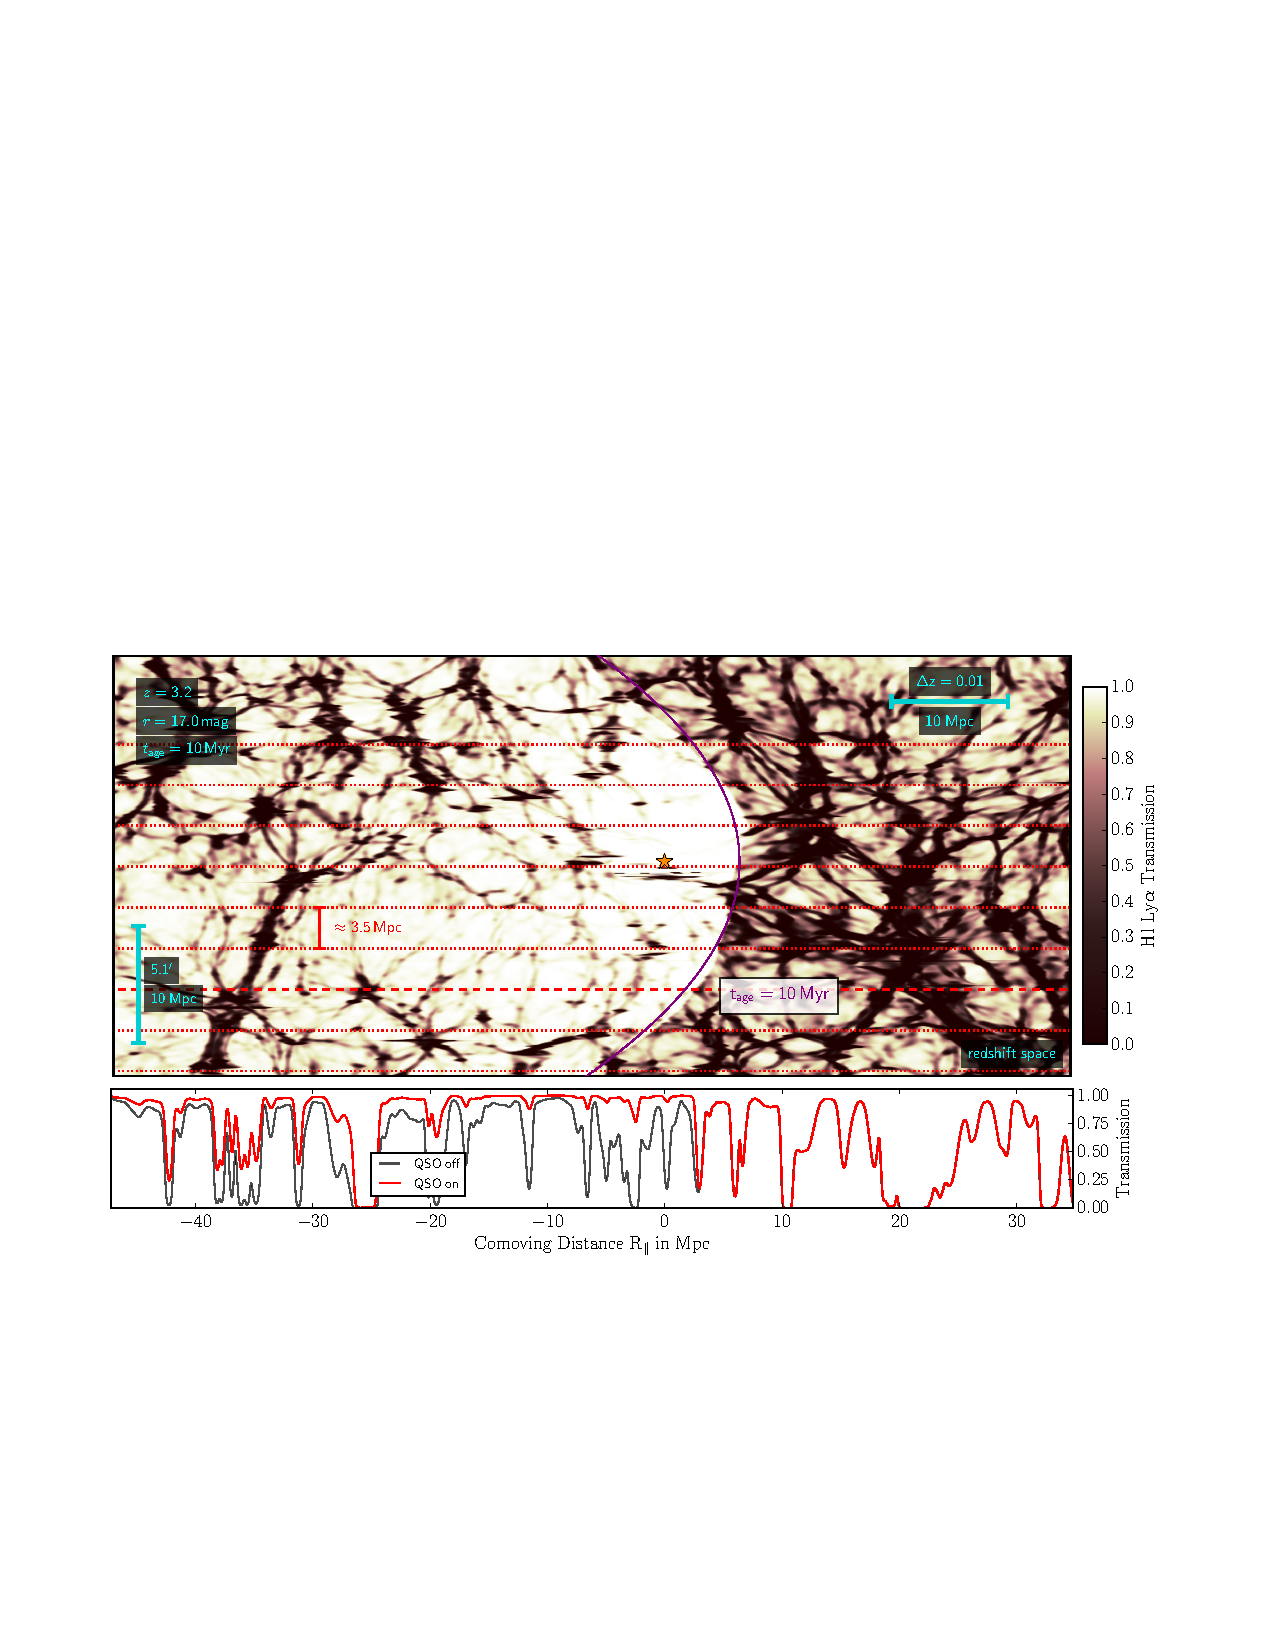
\includegraphics[width=\textwidth]{figs/qso_LightEcho_v1.pdf}
%%
%\caption{{\it Top}: Quasar ``Light Echos'' revealed in a simulated tomographic IGM map in the immediate environs of a quasar (gold star) with several sightlines indicated \citep[from][]{2018arXiv181005156S}.  {\it Bottom}: The ionizing flux within the echo's extent enhances transmission of Ly$\alpha$ photons impinging on absorbers along the line-of-sight.}
%%
%\label{fig:LightEcho}
%%
%\end{figure}

\subsection{The galaxy ecosystem at $z$$\sim$2}
\label{sec:z2galaxies}

With surveys like MOSDEF \citep{kriek15} and KBSS
\citep[e.g.,][]{steidel14}, MOSFIRE has provided powerful new
insights into early galaxies at the $z \sim 2$ peak formation epoch.
A complete picture of the galaxy ``ecosystem'' at this key epoch,
however, must include their gas-filled environments as well. Using
Ly$\alpha$ absorption in background galaxies, a tomographic map of
the intergalactic medium (IGM) in regions surveyed by MOSDEF and KBSS
is a key first step. Its promise and application was demonstrated at
Keck by \citet{lee14}, which motivates FOBOS's UV sensitivity, target
flexibility and multiplex in service of tomographic mapping of
large-scale structure, including protoclusters \citep{lee16}, voids
\citep{krolewski18}, and filaments \citep{horowitz19}.
\citet{2018arXiv181005156S} take IGM tomography in a new direction,
demonstrating with simulated observations that quasar ``light echos''
--- spatial signatures of the expanding ionization front of a newly
activated quasar --- can be detected and used to infer opening angles
and deconstruct the quasar's accretion history (see Fig
\ref{fig:LightEcho}). The required FOBOS spectra can simultaneously
constrain the C IV mass density (via $\lambda\lambda$ 1548, 1550 \AA)
and patterns of C IV enrichment on both IGM and cicumgalactic scales,
revealing the imprint of galaxy fueling and feedback processes
\citep[e.g.,][]{tumlinson17}.

%The volume density and chemistry of gas in between galaxies
%\noindent\comment{Hennawi, KG, Prochaska, Burchett: comments? further material to add?}

% \subsection{Ly$\alpha$ morphology and kinematics of lensed, magnified galaxies at $z$$\sim$2--3}

% \noindent\comment{Siana}

% \subsection{The budget of ionizing photons at $z$$\gtrsim$2.5}

% \noindent\comment{Shapley, Siana}


% From George:
% - fill out case for probing both galaxies and their “gas-filled
%   environments”
%    - make it more explicit that getting large numbers of redshifts
%      would make it possible to trace out large-scale structure in
%      detail
%    - enables studies of galaxy properties as a function of environment
%
% - also mention targeting galaxies along QSO lines of sight
%    - much higher target density than with LRIS, DEIMOS over larger FOV.
%
% - Worth discussing Lyman-alpha or metal-line tomography?  
%
% - More quantitative comparisons with existing data sets?
%    - What key science questions can FOBOS address that many years of
%      LRIS and DEIMOS observations have not been able to?  Surely some
%      level of the spectral tagging and photo-z training can be done
%      (and surely is being done) with existing data.  Is FOBOS going to
%      be a huge leap, or will it mainly be cleaning up neglected corners
%      of parameter space?
%
% - More excited to hear about how the FOBOS spectra will be used for
%   science directly, instead of support for LSST

%-----------------------------------------------------------------------


%%%%
% -- Cosmology Science
% --     FOBOS Keck White Paper 2019
%%%%

\subsection{Enhancing Dark Energy Probes via Precision Cosmic Distances.}
\label{sec:cosmology}

Panoramic imaging surveys --- culminating in LSST, Euclid, and WFIRST --- are seeking to constrain the dark-energy
equation-of-state at $z \lesssim 1$ through measurements of angular correlations of galaxy positions, their
gravitational lensing shear, and the cross-correlation between the two.  These surveys rely on photometric redshifts
(``photo-$z$s''), whose uncertainties and potential biases are the major limitation and source of systematic error in
these efforts.  \citet{newman15} define a \emph{spectroscopic} survey for photo-$z$ training that would \emph{increase
the dark energy figure-of-merit in LSST by 40\%}.  The survey program is ideally matched to FOBOS.  It requires 10
independent fields, each 20 arcmin in diameter, with a sampling density of 6 arcmin$^{-2}$, and the ability to go very
deep ($i_{\rm AB} < 25.3$).  FOBOS's lack of a ``redshift desert'' further eliminates the need for expensive, space-based\footnote{Ground-based near-IR spectroscopy is too contaminated by
sky-line emission to provide spec-$z$s at the required level of completeness \citep{newman15}.} near-IR spectroscopy to train photo-$z$s with $z > 1.5$.  Highly accurate photo-$z$s will enable science applications with massive imaging surveys that go beyond cosmology.

\subsection{Cosmology with LBG--CMB cross correlation.}
\label{sec:LBG}

High-S/N CMB maps from next-generation CMB observatories (e.g., Simons Observatory and CMB-S4) will provide a cosmic
``reference background'' for measurements of gravitational lensing induced by matter along the line of sight.  After
cross-correlating with Lyman Break Galaxy (LBG) samples, a relatively flat lensing ``kernel'' with power at $z = 2$--5
enables powerful constraints on the Inflation-sensitive matter power spectrum, Horizon-scale General Relativity, cosmic
curvature and neutrino masses, and early Dark Energy.  \citet{wilson19} explore these constraints in detail and
highlight the need for spectroscopic determination of accurate redshift distributions for the employed LBG samples.
FOBOS would address this need in two ways.  First, several deep-drilling fields targeting $\sim$1000 LBGs BX, $u$, $g$,
and $r$ drop-out candidates per pointing ($\sim$10,000 deg$^{-2}$) would establish the interloper rate and intrinsic
redshift distribution of LBG samples to sufficient precision (this program would likely overlap with the photo-$z$
program described above).  Second, $\sim$200 LBGs per pointing (2000 deg$^{-2}$) could be included as a background
program when FOBOS observes other sources across the sky, eventually building a 50-100 deg$^2$ survey of sparse
high-$z$ spectroscopy for LBG dN/d$z$ calibration via clustering redshifts \citep[see][]{wilson19}.



\noindent\comment{Kinematic Weak Lensing: Bundy, Huff, Schlegel, DiGiorgio?}

%%%%
% -- Data Science
% --     FOBOS Keck White Paper 2019
%%%%

\subsection{FOBOS as an ideal spectroscopic training instrument}
\label{sec:datascience}

FOBOS will provide observations that directly lead to invaluable
science. However, FOBOS will also allow teams of Keck scientists to
quickly build spectoscopic samples purposely designed to be used in
training machine-learning algorithms. These data will allow us to
statistically infer physical properties from upcoming large-scale
broad-band imaging surveys (e.g., LSST, WFIRST, Euclid) that are only
directly accessible via spectroscopy and complement more shallow
spectroscopic surveys made with FOBOS or surveys using smaller
aperture facilities (e.g., APOGEE, DESI). Keying off one of NSF's ten
Big Ideas, we highlight a few ways that FOBOS can be used to "harness
the data revolution."

\comment{these sections need to be shortened}

\begin{figure}[h!]
%
\vskip -0.1in
%
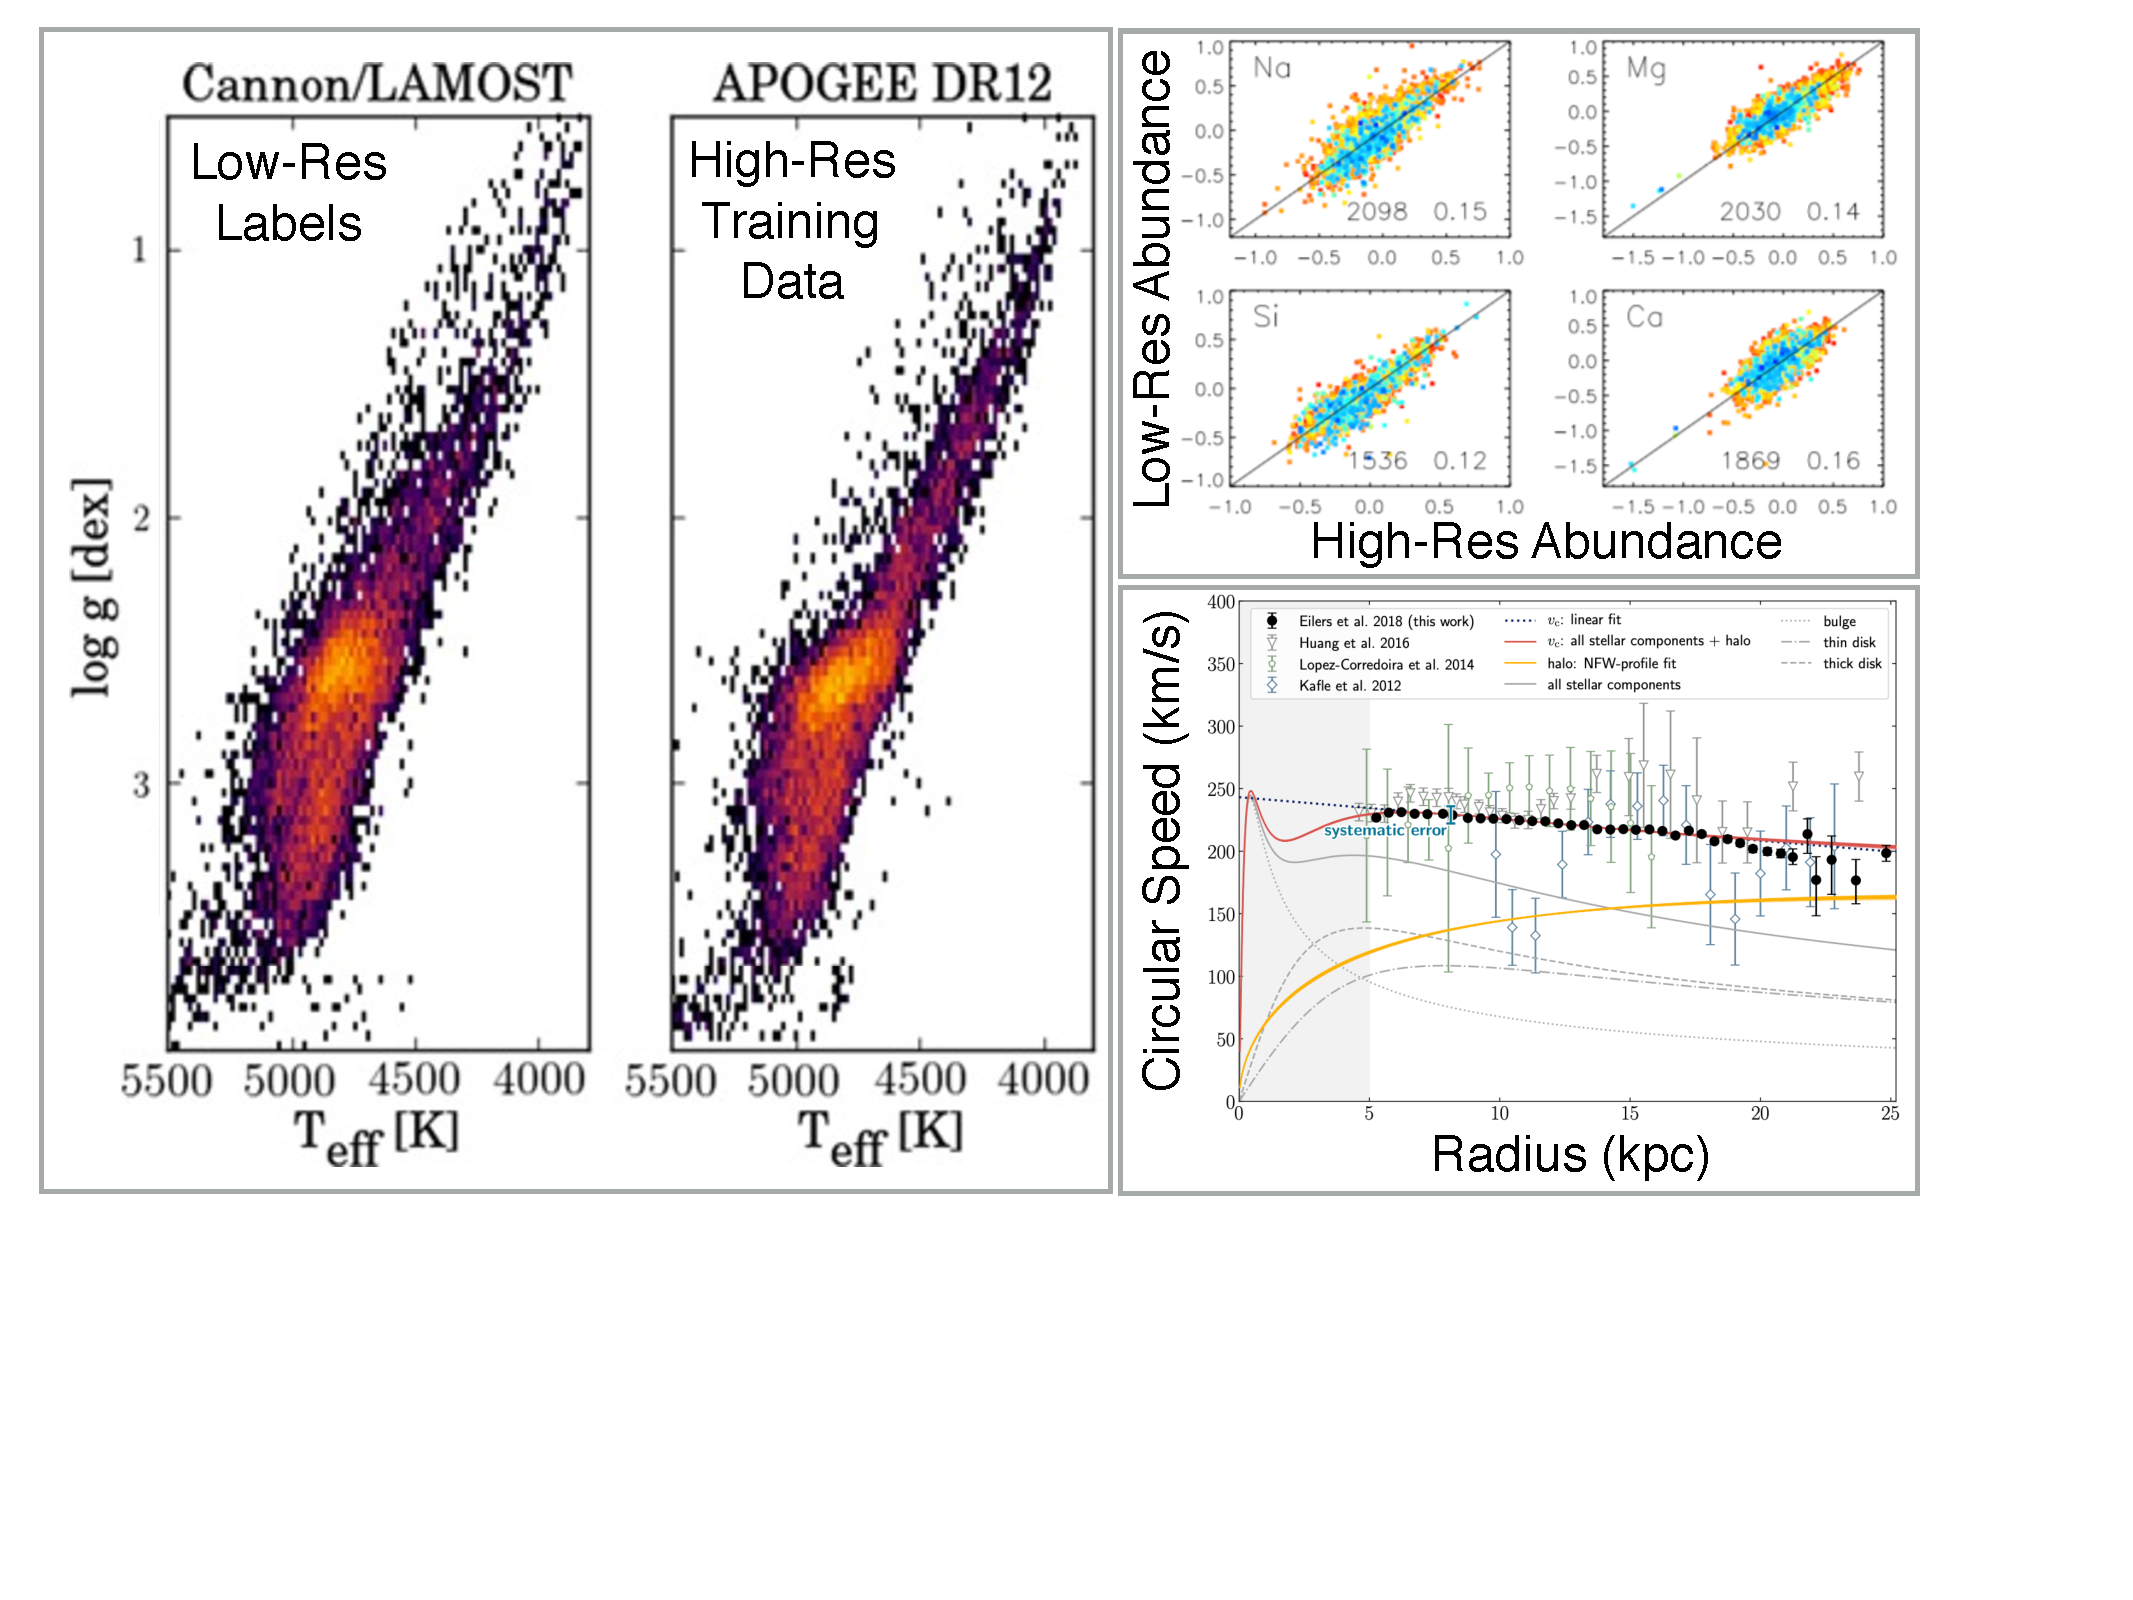
\includegraphics[width=\textwidth]{figs/LGplots.pdf}
%
\caption{{\it Left}: Validation of {\it The Cannon} measurements of
stellar effective temperature, $T_{\rm eff}$, and surface gravity, $\log
g$, using low-resolution LAMOST spectra (left) compared to
high-resolution APOGEE measurements
\citep[right;][]{2017ApJ...836....5H}. {\it Top-right}: Recovery of
elemental abundances from low-resolution LAMOST spectra compared to
high-resolution measurements from GALAH (Xiang et al., in prep).  {\it
Bottom-right}: The circular-speed curve of the Milky Way determined
using a data-driven model that combines stellar parameters determined
from APOGEE spectra with photometry from WISE, 2MASS, and Gaia, yielding
the most precise measurements to date \citep{2019ApJ...871..120E}.}
%
\label{fig:Cannon}
%
\end{figure}

\subsubsection{The chemical evolution of Milky Way stellar populations}
Radial velocity studies of stars in the MW halo or the M31 disk require
observations of up to 10 hours on large telescopes
\citep[e.g.,][]{2018arXiv180904082C}.  This again motivates
machine-learning algorithms to extract physical quantities from both
multi-band imaging and lower quality spectra (low resolution and S/N)
using relatively small, yet high-S/N, training sets.  For example,
\citet{2015ApJ...808...16N} have developed {\it The Cannon}, a
supervised learning approach that uses spectra with known stellar
parameters to label spectra where those parameters are unknown
(Fig.~\ref{fig:Cannon}).  Additionally, \citet{2018arXiv180401530T} have
developed {\it The Payne} which can infer 16 stellar-abundance labels
from low-resolution spectra using a neural network and theoretical
stellar spectra.  Finally, \citet{2018arXiv180803278T} have combined
Kepler-based astroseismology measurements with APOGEE spectra to
determine stellar age to $\sim$25\% precision using a neural network.
Our proposed effort builds on new lines of inquiry based on these
successes.

A nested network of stellar parameter training samples for resolved
Milky Way and Local Group studies via extracting maximum information
from photometry, in this case stellar parameters. Our goal is to
reach magnitudes significantly fainter than the detection limit of
current and upcoming spectroscopic surveys of the Milky Way including
Gaia, APOGEE,\footnote{APOGEE, the Apache Point Observatory Galaxy
Evolution Experiment has observed in both SDSS-III and SDSS-IV.} the
SDSS-V Milky Way Mapper, planned programs with 4MOST\footnote{4MOST:
4-meter Multi-object Spectroscopic Telescope.} and the Dark Energy
Spectroscopic Instrument (DESI) Milky Way Survey, among others.
Inferring stellar parameters beyond V$\sim$18 will open up studies of
the Milk Way's outer halo, the halo of M31, and stellar populations
in local dwarf galaxies.

The immediate challenge is to design an optimized, nested set of
training samples that connect data from the surveys above. This
nested set will span high-S/N to low-S/N and high spectral resolution
to low spectral resolution for sufficiently large, overlapping
stellar samples. Subsets will have astroseismology from
TESS\footnote{TESS is NASA's Transiting Exoplanet Survey Satellite.}
and PLATO.\footnote{PLATO is ESA's PLAnetary Transits and
Oscillations mission.} Using simulated spectra with known input
parameters, we will test methods for ``label transfer'' from
information-rich spectra to information-poor spectra as we work down
to fainter magnitudes, landing eventually at multi-band photometry
alone. Within this nested set, low-resolution FOBOS data will fill in
gaps at both high-S/N, where we will be training FOBOS data on higher
resolution spectroscopy, as well as lower-S/N where we will be
training photometry on FOBOS spectroscopy. The success of this
multi-layered label transfer depends not only on the size of the
training sets we can access or observe, but on how representative
they are. Label transfer to WFIRST imaging of the M31 halo, or Local
Group dwarfs in either hemisphere, is a particular concern. We will
test it by evaluating label recovery on simulated stellar spectra
with cosmologically informed formation histories for M31 and dwarf
galaxies, suitably differentiated from the Milky Way stars that
anchor the training network.

\comment{Raja, Ting: Help with shortening/refocusing the above}

\subsubsection{The $z$$\sim$2 Galaxy Population}

For decades, we have used the spectral information encoded in
broad-band photometry to infer properties of galaxies beyond their
color and brightness. The most common application is to estimate the
galaxy redshift from its broad-band colors, i.e. photometric
redshifts (photo-$z$s). However, as demonstrated in Figure
\ref{fig:SOM}, the range of observed spectral types is
well-constrained by broad-band imaging, suggesting a far greater
potential for imaging data to reveal physical properties with
sufficient training of deep-learning algorithms.  These properties go beyond what conventional modeling of spectral energy
distributions (SEDs) would suggest. The challenge here is to identify
the extent to which machine learning can deliver SDSS-like
information --- e.g., star-formation histories, stellar-population
properties, dust content, inflow/outflow properties, and stellar
masses --- and determine design parameters for future training sets
that will enable such inferences for millions of imaged galaxies at
$z$$\sim$2.

Self-Organizing Maps (SOM, Figure \ref{fig:SOM}) provide a
state-of-the-art representation of a high-dimensional input space in
projected 2D grid cells, allowing us to benchmark sampling of the
photometric color space under various training set designs. We will
also use Bayesian Optimization techniques to evaluate the success of
simulated training sets against the fidelity of full cosmological
analyses that employ them. This will enable extremely rapid
exploration of the optimal design space.

\comment{Master, Mandelbaum, Rau, Schafer}

\begin{figure}[h!]
\vskip -0.1in
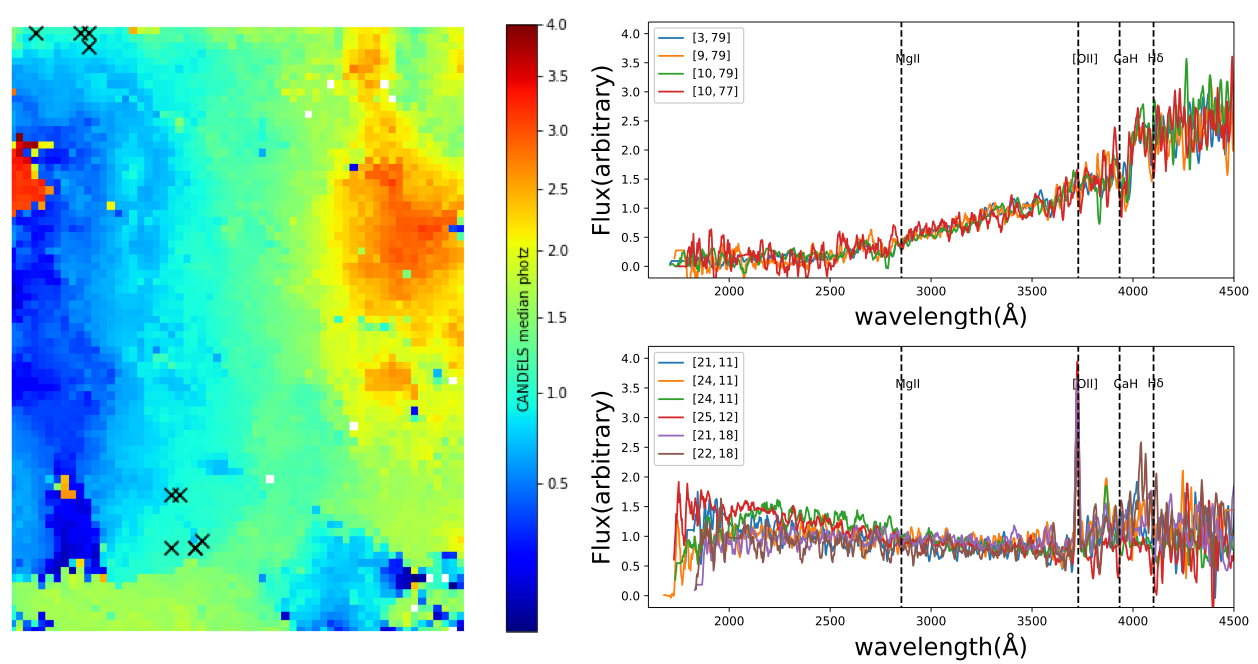
\includegraphics[width=\textwidth]{figs/Hemmati18_Fig8_VVDS_spec.png}
\caption{\small {\it Left}: A Self-Organizing Map
\citep[SOM;][]{1990Natur.346...24K} from \citet{hemmati18} encoding
the relation between colors in an LSST+WFIRST-like color space and
redshift, $z$. Position in the SOM is associated with a position in
the multi-dimensional broad-band color space of galaxies. Galaxies
observed in this space are assigned $z$ values based on the median
photo-$z$ of galaxies from the CANDELS survey \citep[color
bar;][]{2011ApJS..197...35G}. Such SOMs can be used to optimally
define spectroscopic training samples for use with imaging surveys.
{\it Right}: Galaxy spectra from VVDS \citep{2005A&A...439..845L};
black crosses near the top and bottom of the SOM are plotted in the
top and bottom panels, respectively. Note the similarity of the
high-resolution spectra associated within the SOM, suggesting that a
systematic spectroscopic exploration of the LSST color space would
have far-reaching benefits to the science return of the mission
beyond the photo-$z$ application.}
\label{fig:SOM}
\end{figure}

% The complete photo-$z$ training survey described in \citet{newman15}
% would require 15 independent pointings, each spanning 0.1 deg$^2$ with
% a target density of 6 arcmin$^{-2}$ (8 arcmin$^{-2}$ when including $z
% > 1.5$ galaxies accessible in the UV with Keck-FOBOS), perfectly
% matched to the Keck-FOBOS field-of-view and target density.  With a
% conservative exposure time of 100 hours to reach 75\% redshift
% completeness for 40,000 galaxies with $i_{\rm AB} < 25.3$, the Neman
% survey would require 400 nights.  Challenge \ref{photoz} would reduce
% the required survey duration by a factor of at least four.  Meanwhile
% the extreme depths and flux-limited selection are likely also
% requirements for training sets associated with Challenges \ref{phot},
% \ref{uv}.

% A wider and shallower survey component is envisioned for Challenges
% \ref{lowsnr} and \ref{gaia}.  With 10-minute integrations, a 52
% deg$^2$ Keck-FOBOS sample of environmental diagnostics for 1 million
% galaxies could be carried out in less than 20 nights.  This program
% would sample at $z \sim 1.5$ the same cosmic volume as SDSS.  A
% program of a similar scale would provide training set data for
% inference of stellar parameters in the Milky Way.  These shallow
% programs would be integrated with the deeper components described
% above into a single survey plan.

%%%%
% -- Instrument Description
% --     FOBOS Keck White Paper 2019
%%%%


\section{FOBOS Instrument Description}
\label{sec:concept}
% \noindent \comment{1 page}

% Here's an alternative way to put in figures if we want captions on the side (to save space)
% Could introduce a new ``counter'' to count and label figures appropriately
%\centerline{\hbox{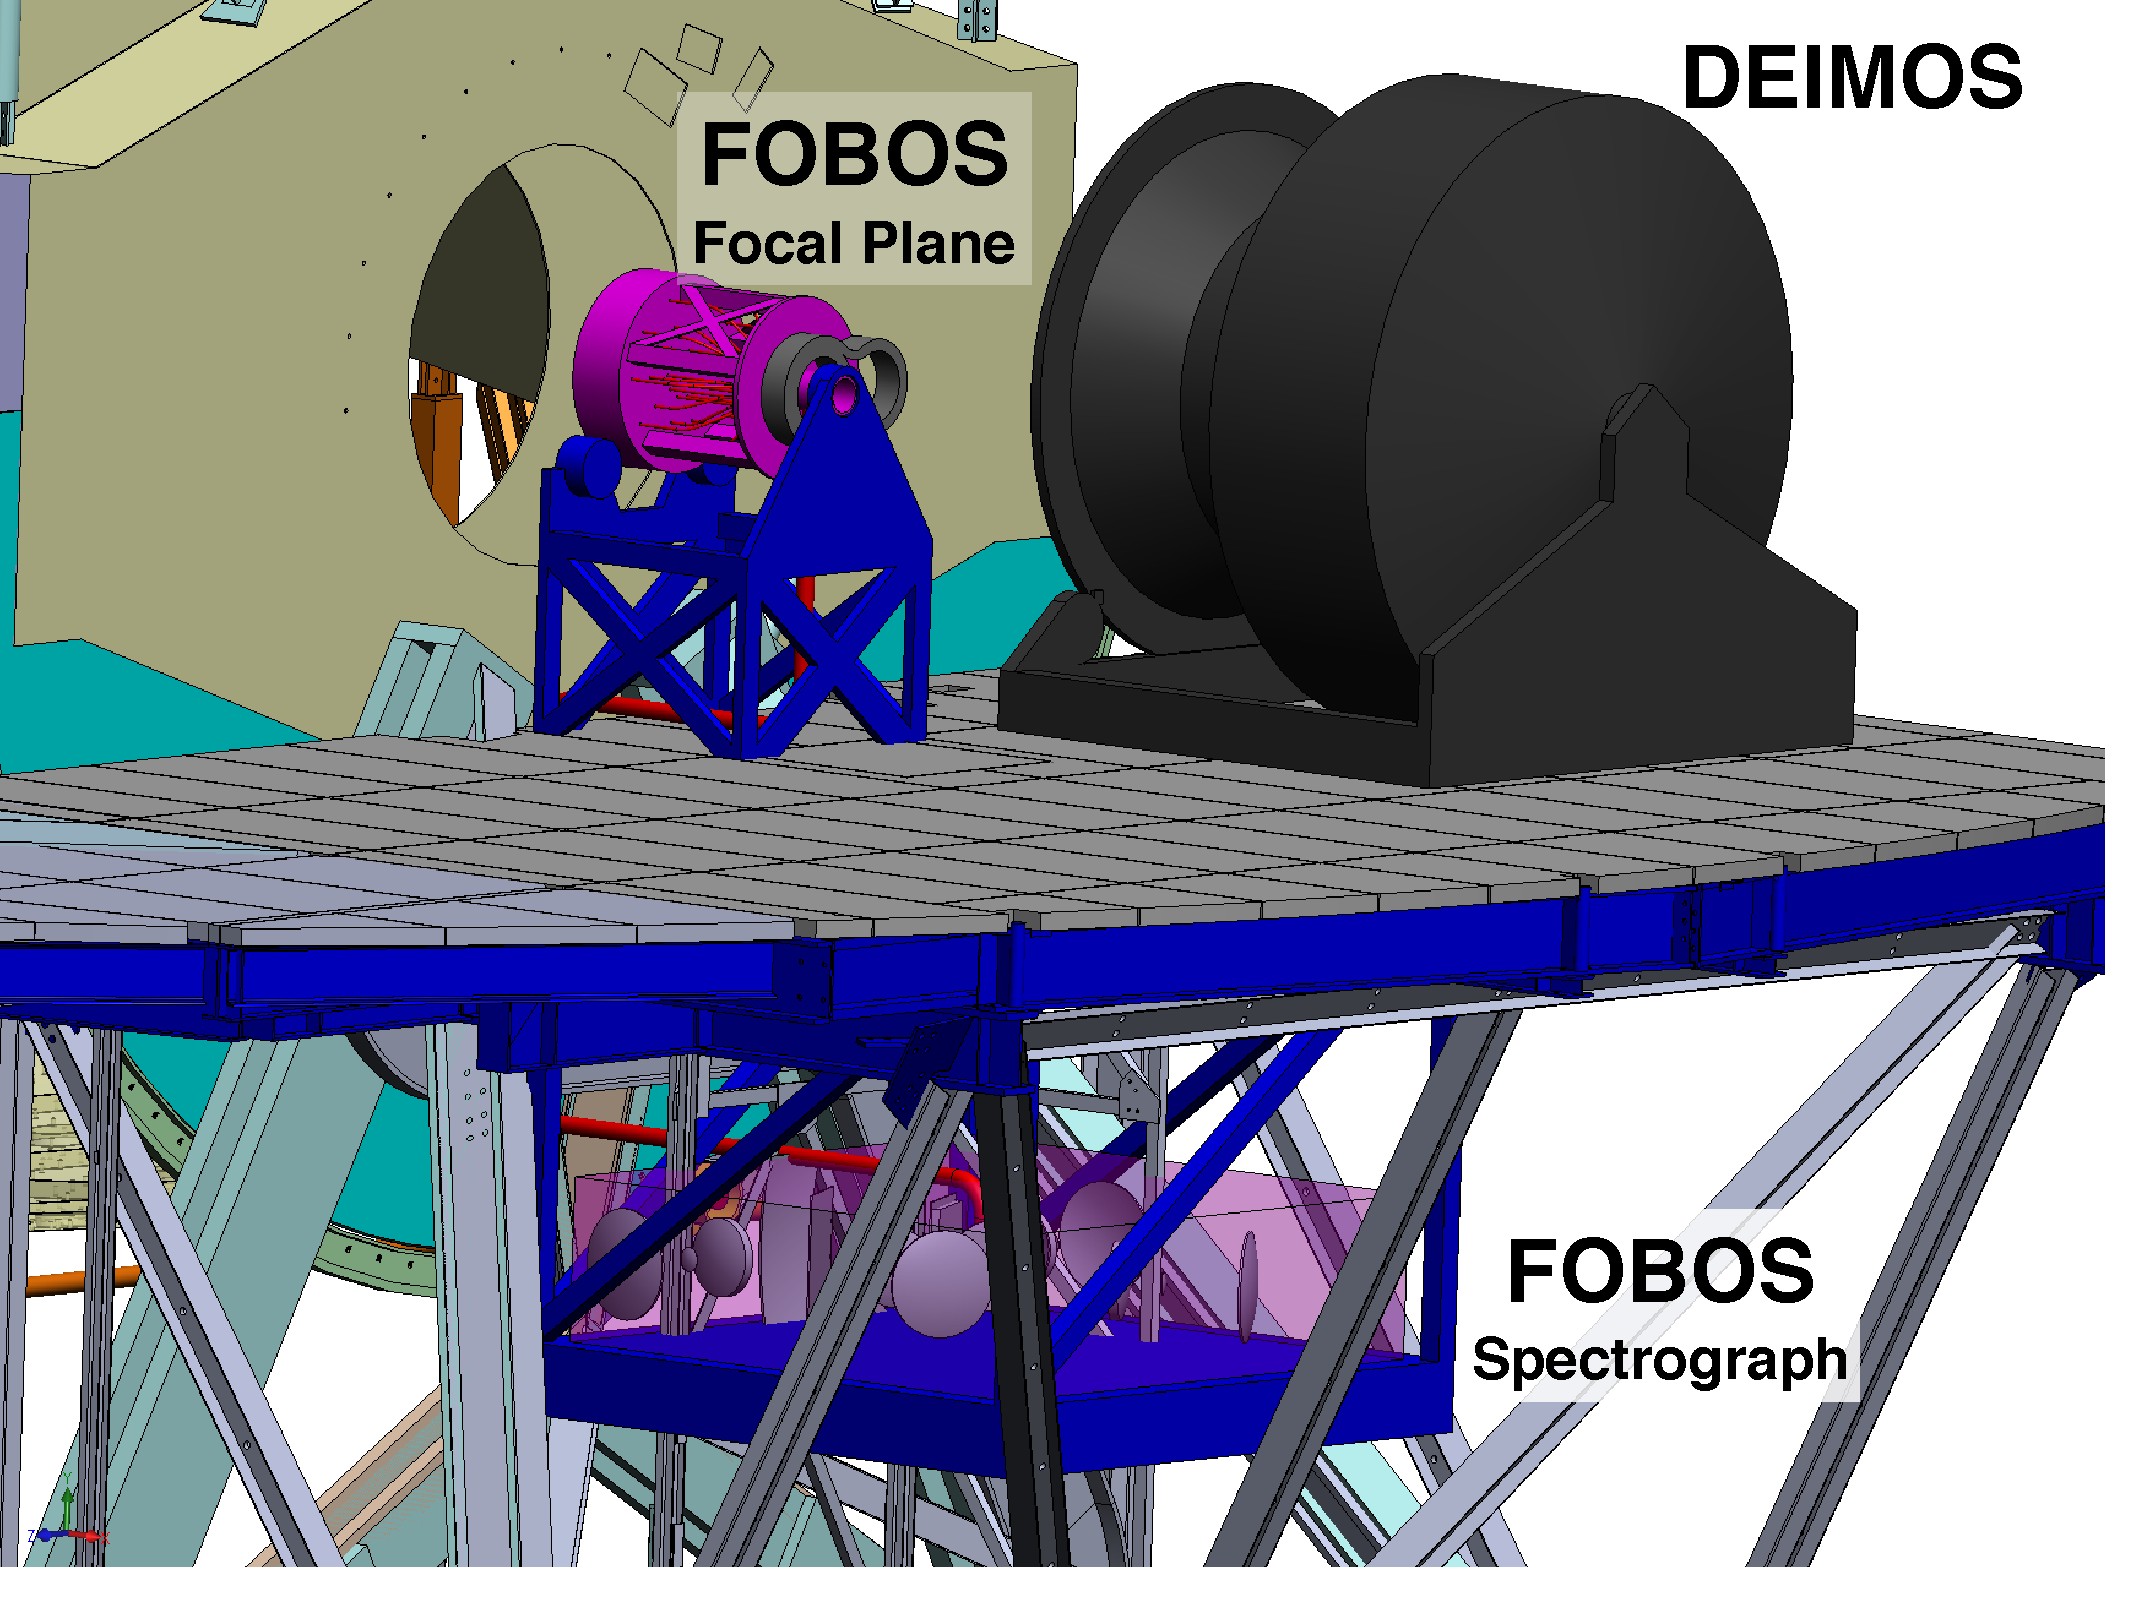
\includegraphics[width=0.6\textwidth, angle=0]{figs/FOBOSatKeck_v1.pdf}
%    \hspace{0.1cm} \vspace{2in}
%    \parbox[b]{0.3\textwidth}{\small {\bf Figure ??:} Rendering of FOBOS instrument systems deployed at the Keck II Nasmyth port.  By mounting the FOBOS spectrographs under the Nasmyth platform, other instruments like DEIMOS can maintain access to the telescope. \vspace{2cm}}}}

\begin{figure}[h!]
%
\vskip -0.1in
%
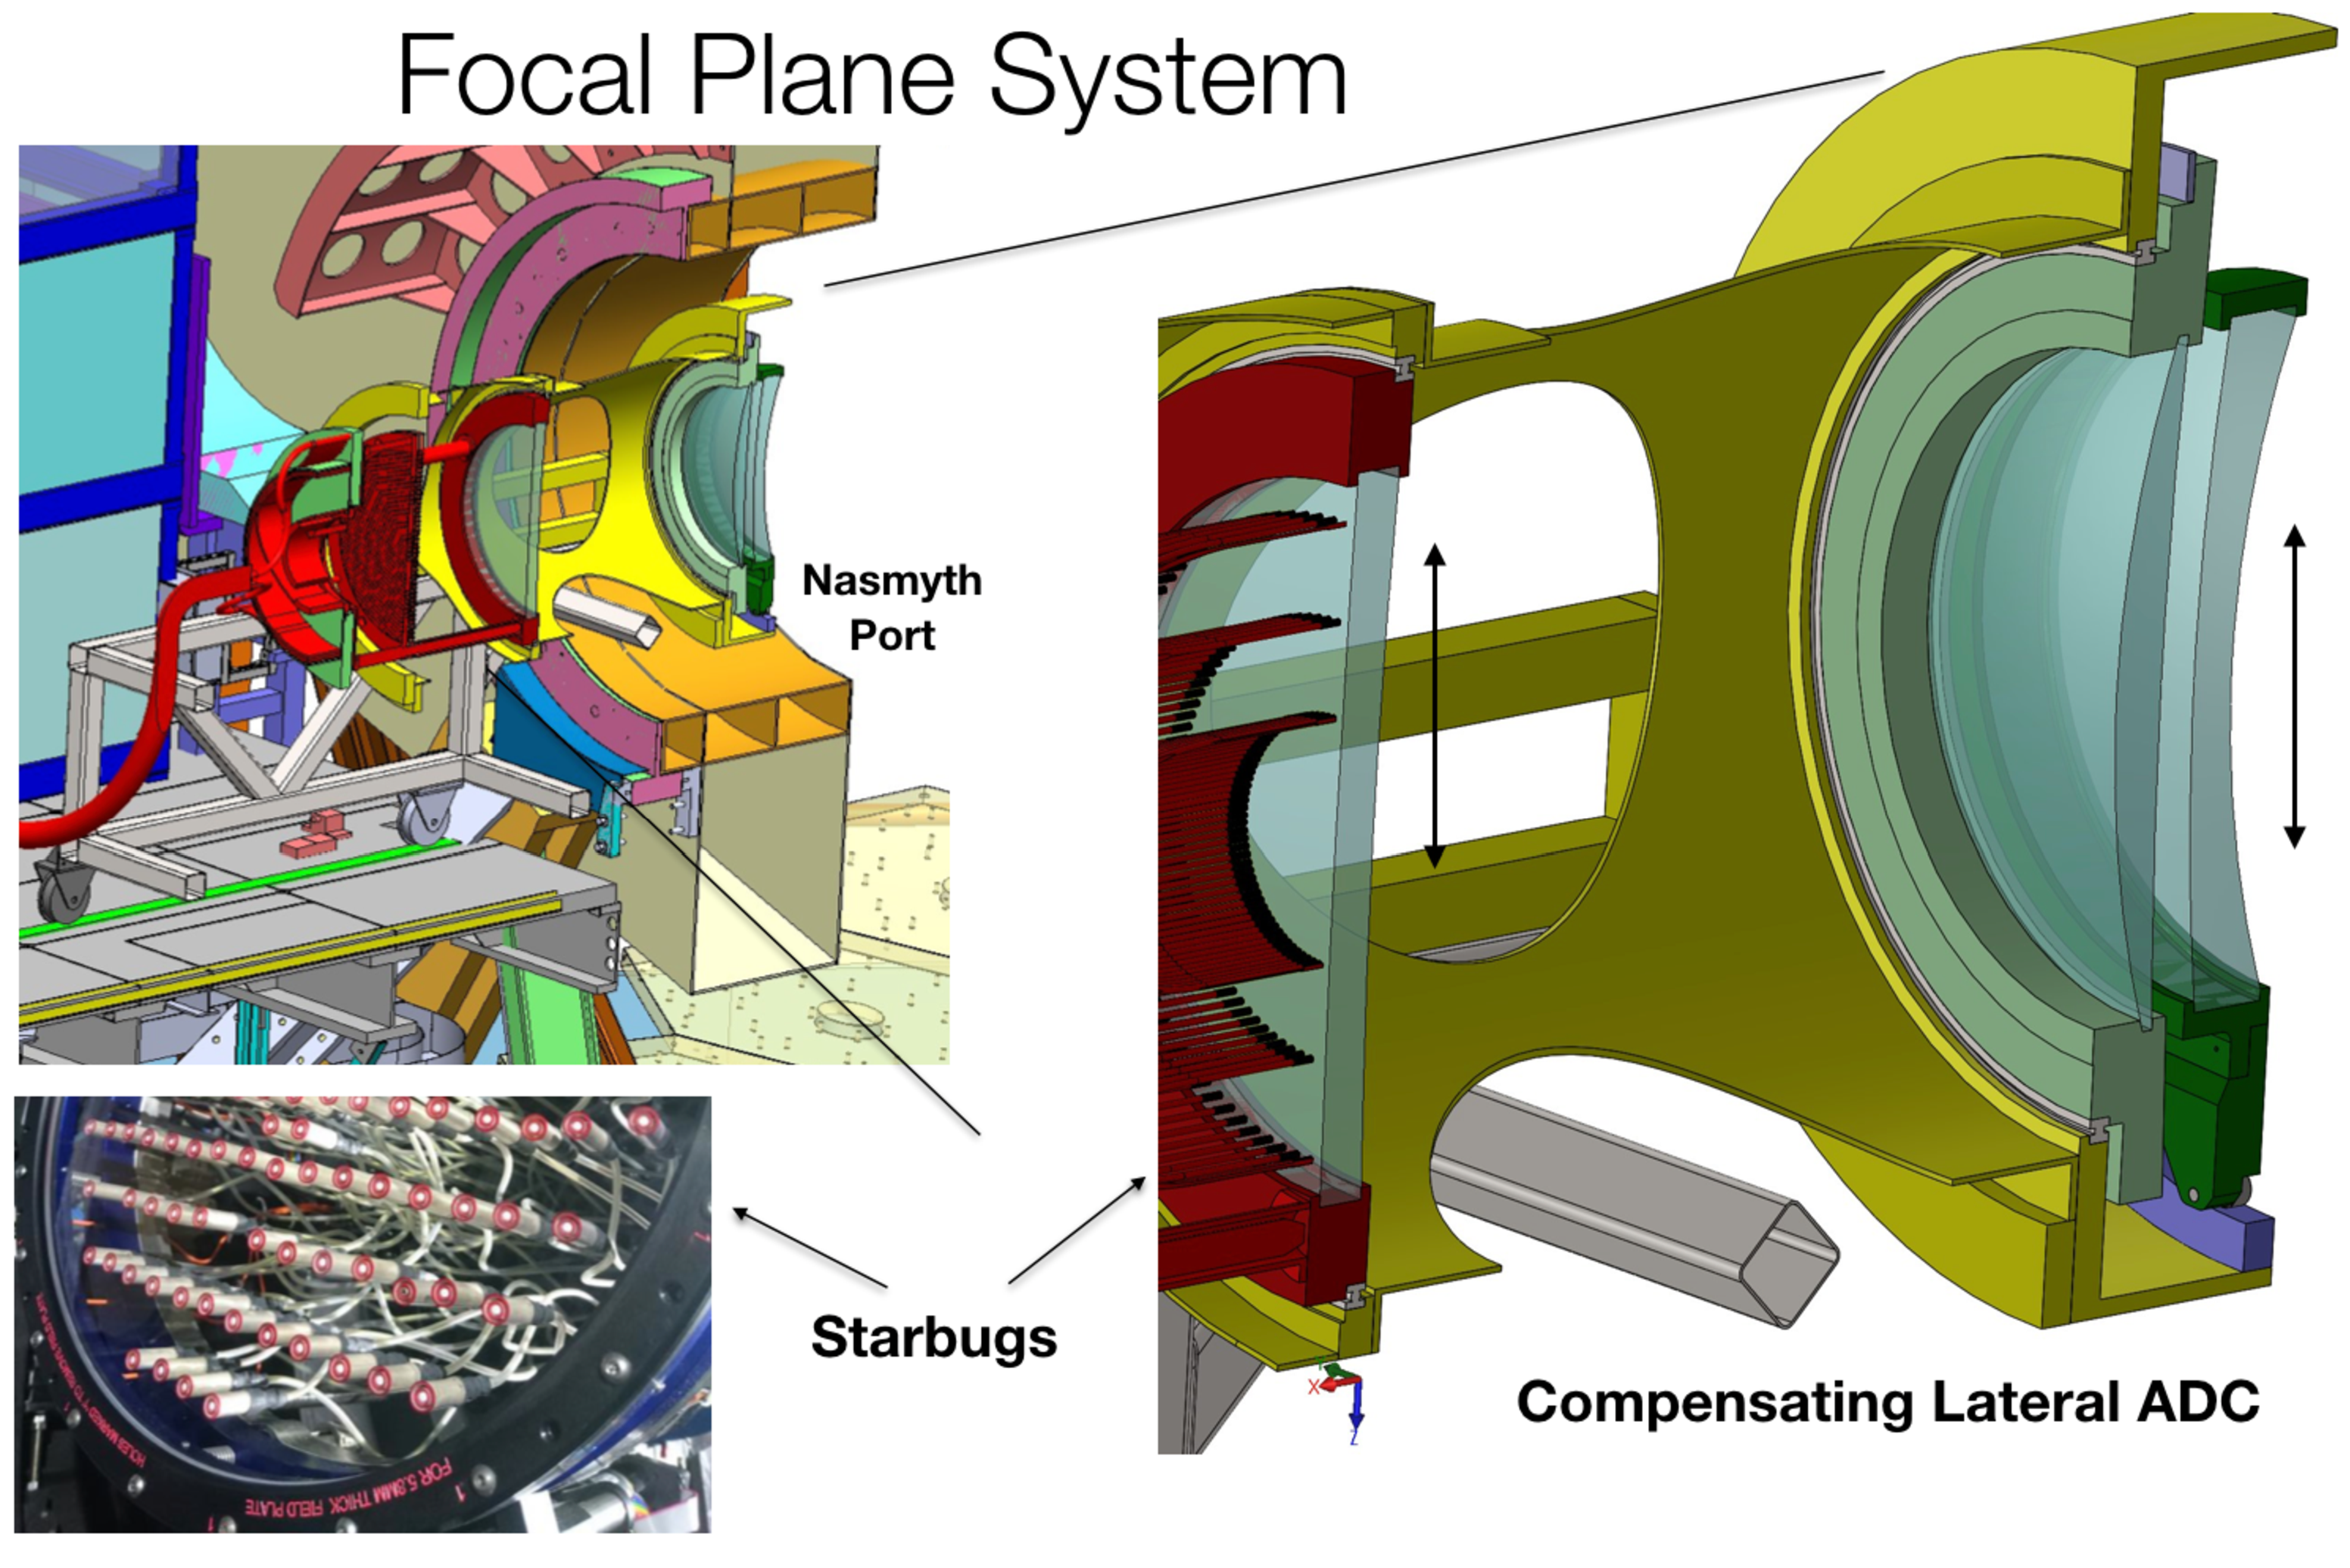
\includegraphics[width=\textwidth]{figs/FOBOS_FocalPlane.pdf}
%
\caption{\small {\it Left}: Rendering of FOBOS focal plane system
deployed at the Keck II Nasmyth port.  By mounting the FOBOS
spectrographs under the Nasmyth platform, other instruments like DEIMOS
can maintain access to the telescope. {\it Right}: Rendering of the ADC and focal surface with Starbugs mounted (red cylinders).  {\it Bottom-left}: Starbugs deployed on the TAIPAN instrument.}
%
\label{fig:focalplane}
%
\end{figure}

Mounted at the Nasmyth focus of Keck II Telescope at WMKO, FOBOS (Fig
\ref{fig:layout}) will be one of the most powerful spectroscopic
facilities deployed in the next decade.  FOBOS includes a compensating lateral
atmospheric dispersion corrector (CLADC, not pictured) to ensure that
target light from all wavelengths falls on allocated fibers while also
correcting image aberrations at the edges of the 20 arcmin diameter Keck
field.  Each of the CLADC lenses is 946 mm in diameter, the first two
closely spaced with lateral relative motions enabled by three
barrel-mounted actuators.  The final CLADC lens surface serves as the
vertical mounting plate for roaming Starbugs fiber positioners.  It
translates to track focal plane tilt.  Starbugs patrol a large on-sky
area ($\sim$1 arcmin), enabling flexible and dynamic targeting
configurations with adjacent fibers as close as 10 arcsec.

A total of 1800 150-$\mu$m core diameter fibers are deployed at the curved focal plane.  Fore-optics on the front end
of each fiber demagnify and speed up the beam (from f/15 to f/5) for better coupling to the fiber numerical aperture
and to minimize losses from focal ratio degradation.  The focal plane plate rotates and translates to follow image
positions as the telescope tracks across the sky.  The fiber run is kept at less than 10m to maintain high throughput
at UV wavelengths.  Special care is given to stress-relief cabling to minimize variable focal ratio degradation over
the fiber run.

Sets of 600 fibers feed each of three identical spectrographs (Fig
\ref{fig:layout}).  Each spectrograph uses a series of dichroics to
divide the 259 mm diameter collimated beam into four wavelength channels with combined, instantaneous
coverage from 0.31--1 $\mu$m.  Fused-silica etched (FSE) gratings provide mid-channel spectral resolutions of $R
\sim 3500$ at high diffraction efficiency in each channel.  The dispersed light is focused by an f/1.1
catadioptric camera\footnote{Based on the camera design for the Multi-Object Optical and Near-infrared Spectrograph (MOONS) on the Very Large Telescope (VLT).} and recorded by an on-axis 4k$\times$4k CCD mounted
at the center of the first camera lens element.  Spectrographs are
mounted in a temperature controlled housing installed under the Nasmyth
Deck to allow space for other Keck instruments above.  The end-to-end
instrument throughput peaks at 60\% and is greater than 30\% at all wavelengths
%\comment{compare to PEP}.

FOBOS includes observatory level systems for precise instrument
calibration using dome-interior screen illumination, a metrology system
for accurate fiber positioning, and guide cameras for field acquisition
and guiding.  The instrument design envisions future upgrades including
alternate collecting modes that deploy multiple fiber bundles, feeds to
other fiber-based spectrographs at different wavelengths or spectral
resolutions, and the ability to support and benefit from image
corrections with Ground-Layer Adaptive Optics.


%%%%
% -- Instrument Description
% --     FOBOS Keck White Paper 2019
%%%%


%%%%%%%%%%%%%%%%%%%%%%%%%%%%%%%%%%%%%%%%%%%%%%%%%%%%%%%%%%%%%%%%%%%%%%%%
\begin{figure}[h!]
%\vskip -0.1in
%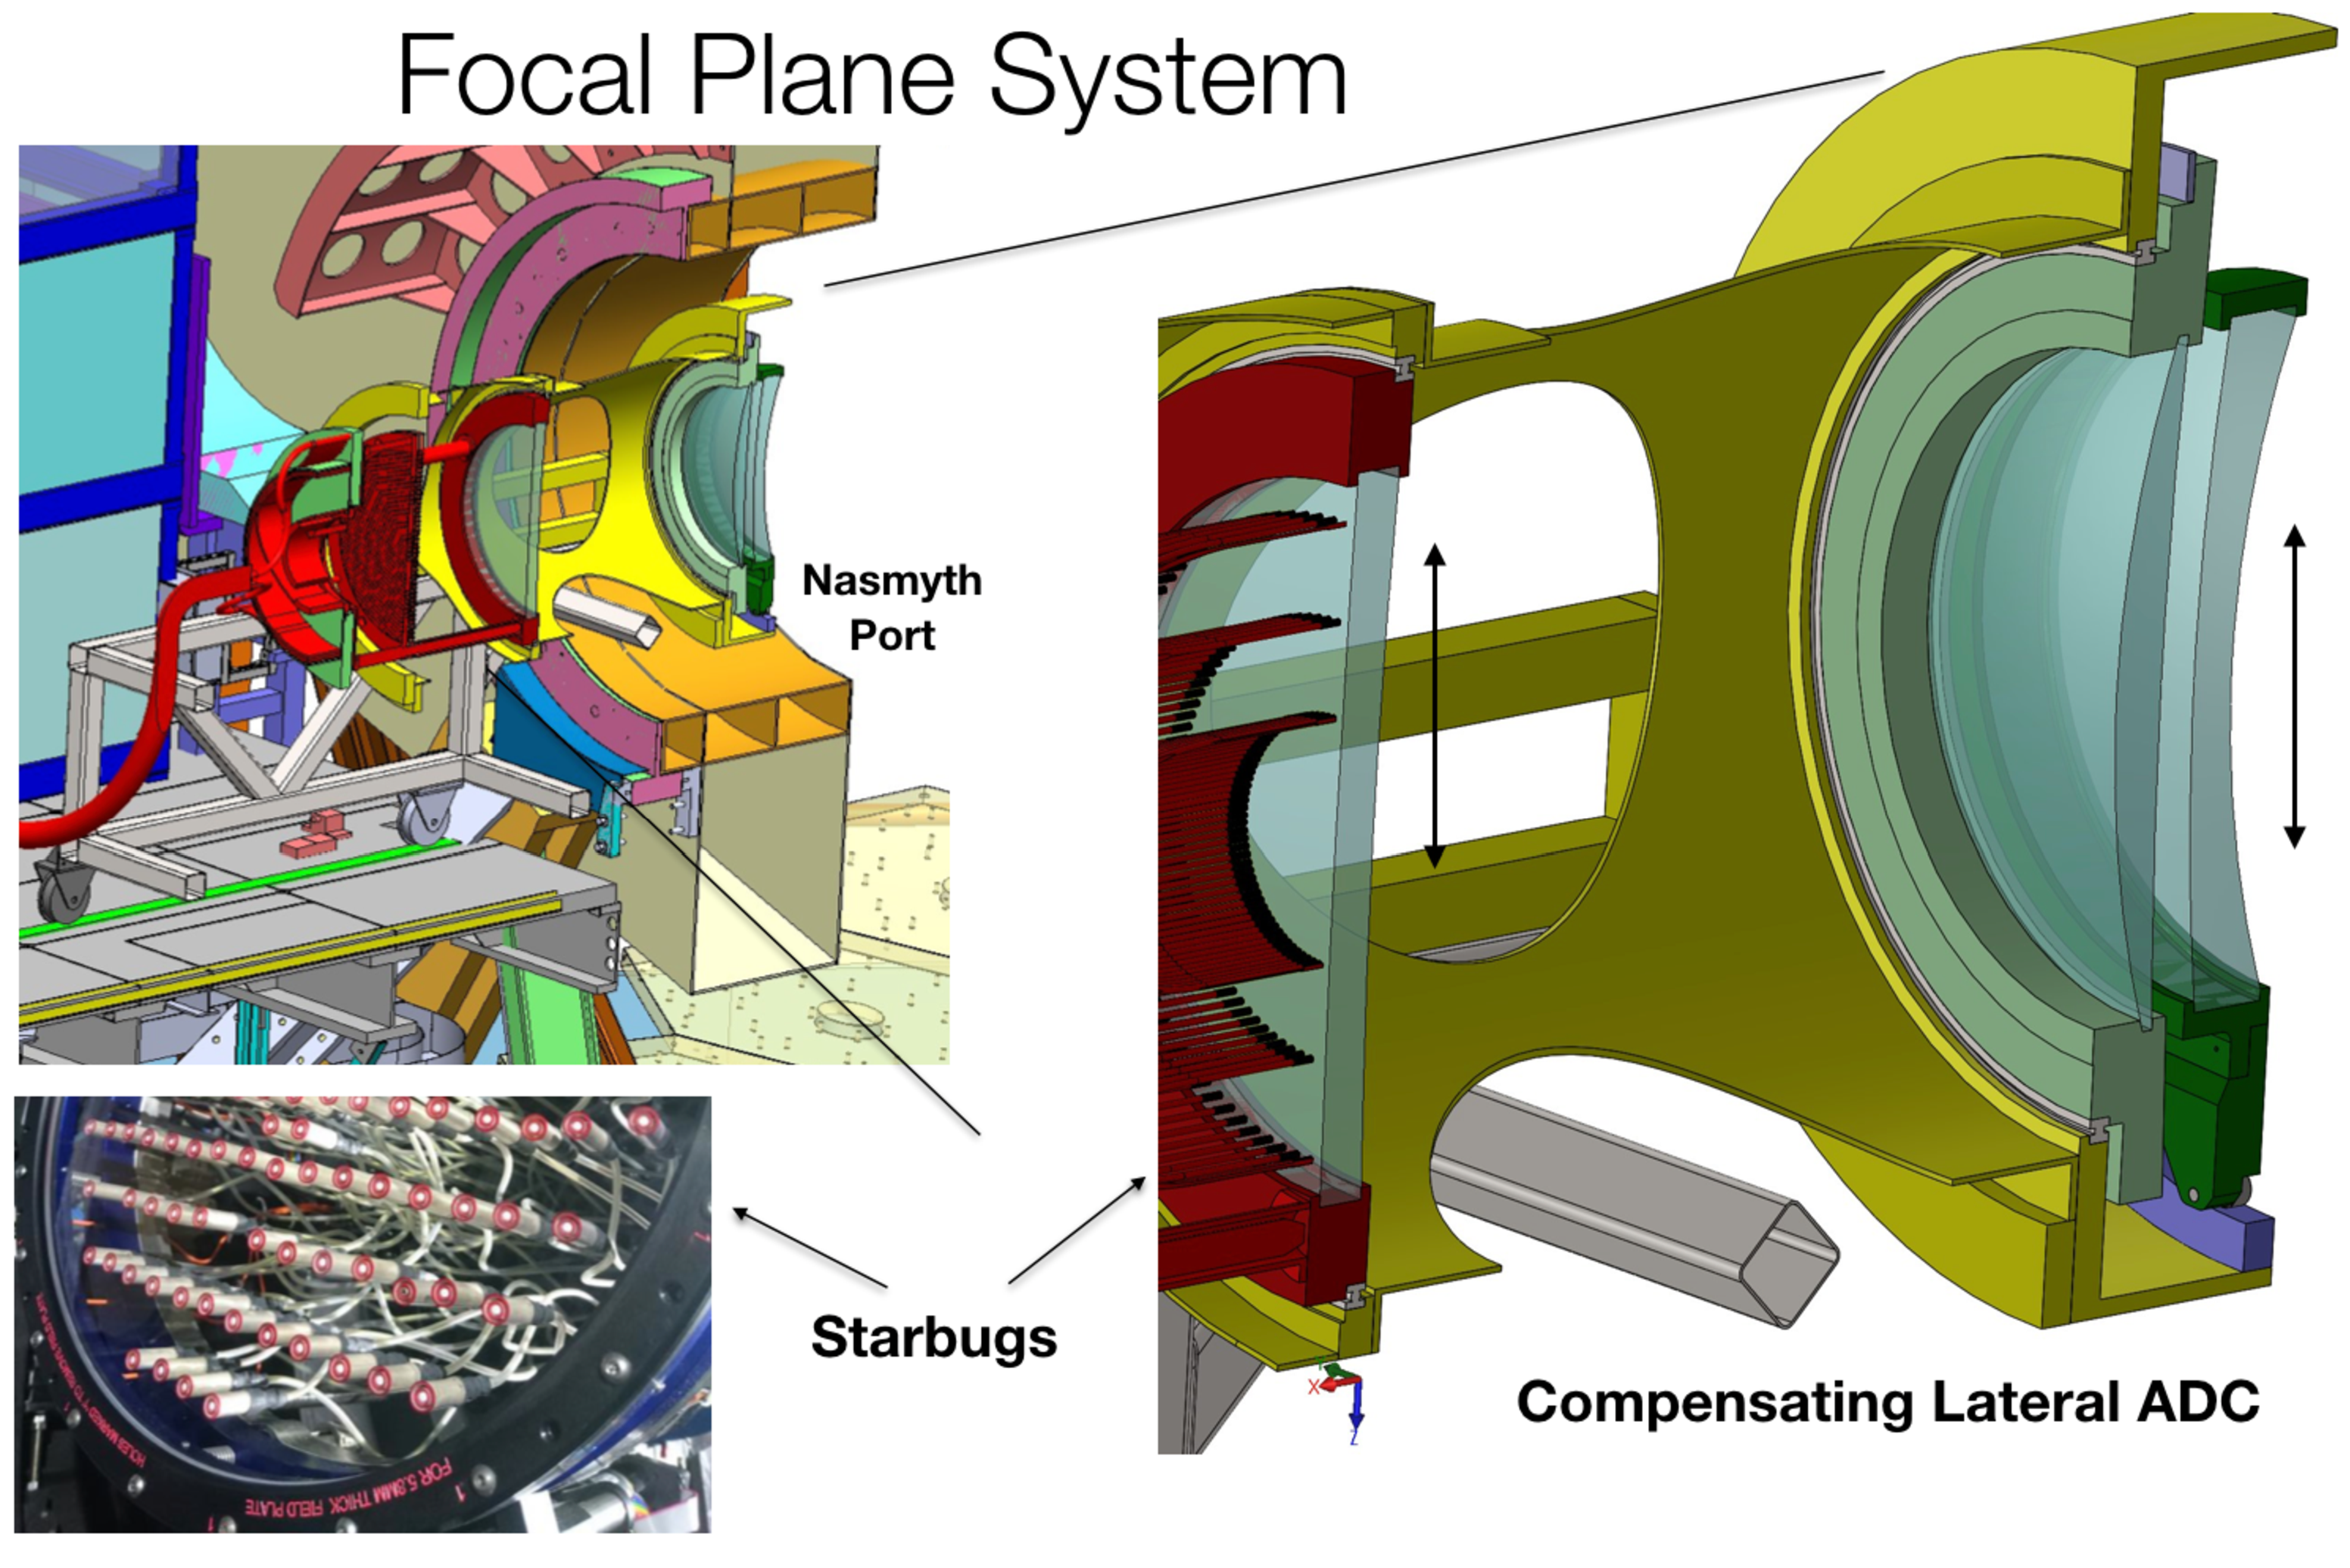
\includegraphics[width=\textwidth]{figs/FOBOS_FocalPlane.pdf}
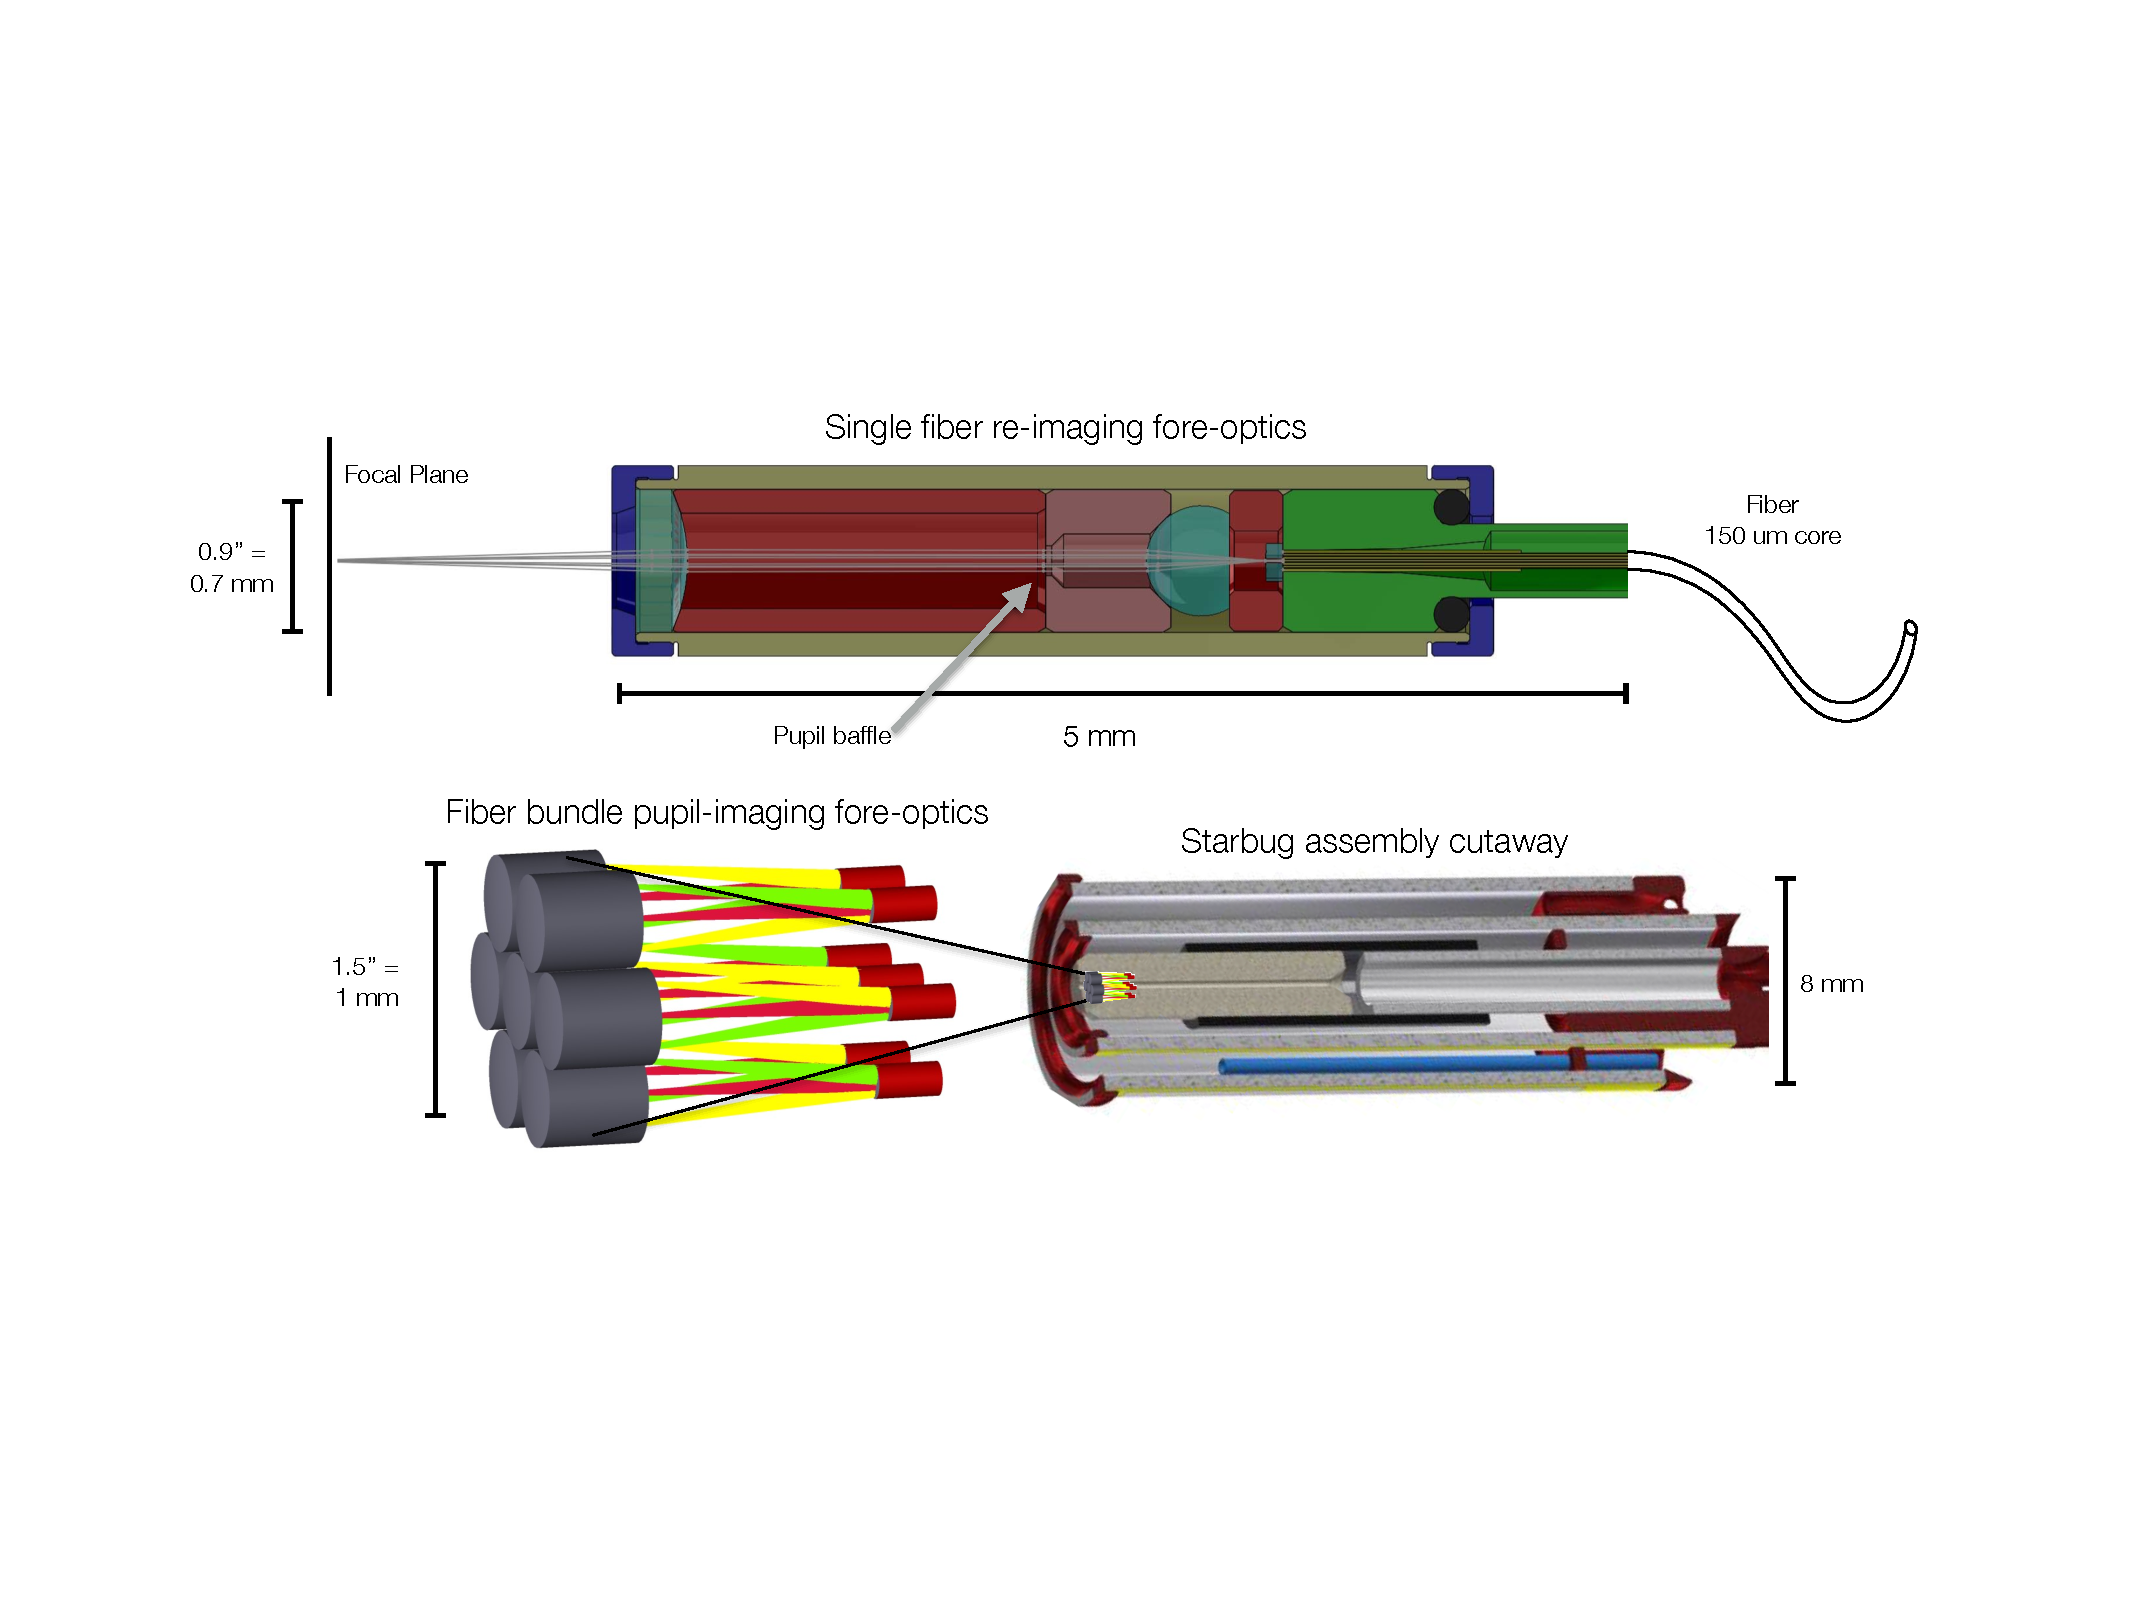
\includegraphics[width=0.9\textwidth]{figs/FOBOS_ForeOptics_v1.pdf}
\caption{\small {\it
Top}: Rendering of fiber coupling fore-optics and mechanical housing for a single fiber using focal-plane re-imaging.  Here the image at the focal plane is demagnified and re-imaged onto the fiber face.  The design allows for a pupil stop. {\it Bottom Left}: Optical layout for a 7-fiber microlens array.  As opposed to focal plane re-imaging, here the telescope pupil is imaged onto each fiber face.  {\it Bottom Right}: In either approach, the fore-optics are housed inside the much larger Starbug, a cutaway diagram of which is shown here. This on-going design work has been funded by the UCO \emph{FIDDLES} project.}
\label{fig:foreoptics}
\end{figure}
%%%%%%%%%%%%%%%%%%%%%%%%%%%%%%%%%%%%%%%%%%%%%%%%%%%%%%%%%%%%%%%%%%%%%%%%


\section{Recent and Ongoing Progress}
\label{sec:progress}

FOBOS development over the past year has focused on (1) engaging the
scientific and instrument-building communities in discussions about
the FOBOS design, particularly with regard to science cases and
instrument feasibility, (2) initial development of an instrument
simulator and exposure-time calculator, (3) advancing the
optomechanical designs of the focal-plane and ADC systems, (4)
consolidating development of Fiber-WFOS for TMT and repurposing much
of the design for FOBOS at Keck, (5) working with Keck instrument
scientists and engineers toward a practical integration plan, and (6)
developing a detailed project execution plan, schedule, and
short-term budget. Many of these activities were enabled by funds
provided in response to our previous white-paper submission.

Visits to Keck-user institutes have been particularly helpful in
building interest around the instrument and refining its
specifications. As of this writing, Bundy, MacDonald, and/or Westfall
have visited UCR (also joined by Michael Cooper from UCI), UCLA, Keck
observatory, LBNL, and UCSB. We plan to continue with visits to UCB, UCD, and CIT before the end of the year.

Feedback from the Keck community has emphasized the desire for very high multiplex, flexibility of the focal-plane
sampling, and sensitivity toward the UV. Although the capabilities of PFS are a common comparison for FOBOS, many of
the science goals now enumerated in Section 1 require target densities and/or wavelength coverage that PFS will not
provide. Another strong message from Keck users was the desire for deployable IFUs. Starbugs are attractive for this
reason becuase they make swapping focal-plane formats straightforward.

% Our
% initial concepts for these different focal-plane formats provided a
% secondary motivation for FOBOS's large pseudo-slit capacity: it can
% provide 15-100 smaller, freely deployable IFUs. Finally, Keck
% remains unique in its throughput toward the atmospheric limit. No
% other current or planned \comment{check this again} spectrograph for
% 10m-class telescopes provides sensitivity below $\sim$380nm,
% providing FOBOS with a unique capability among the landscape of
% forthcoming instrumentation.

% a large-format monolithic IFU and 

% yield a monolithic IFU with a FOV that is competitive with VLT/MUSE
% and can

\subsection{Fiber coupling and Fore-optics}
Another area of progress involves use of UCO funding to address risks in the
coupling of the microlens fore-optics to the fiber and the coupling
of the microlens entrance aperture to the Keck II focal plane (see Figure \ref{fig:foreoptics}).  This ``FIDDLES'' prototyping effort will test coupling performance in labs at UCO and LBL as well as on-sky at Lick and Keck Observatories.  Initial tests have begun and optomechanical designs were recently completed to enable hardware purchases.

% Finally, with the permission of the SSC, we proposed for
% instrument-design funds from the NSF via its new Mid-scale Research
% Infrastructure scheme. Although the proposal was ultimately
% unsuccessful, preparation of the proposal led to a ground swell of
% development in our project planning and science development, much of
% which is included in this submission.

\subsection{New technical expertise from DESI and PFS} Building on the FOBOS instrument team's experience with SDSS projects like BOSS, APOGEE, and MaNGA, we have recruited new expertise from DESI and PFS.  Claire Poppett at SSL/LBNL is DESI's Lead Fiber Scientist and has joined FOBOS to spearhead the fiber system and fore-optics development.  Tim Miller, also at SSL/LBNL, developed the DESI corrector's optical design and will take on the FOBOS ADC.  Renbin Yan, a scientist and instrument builder, has spent the last year at Princeton working with Jim Gunn on PFS-like calibration systems for future instruments.  Renbin was a heavy Keck observer for DEEP2 and will apply PFS knowledge on the calibration problem to Keck and FOBOS.



%%%%
% -- Proposed Work and Budget
% --     FOBOS Keck White Paper 2019
%%%%

\section{Proposed Work}
\label{sec:design}

\subsection{Instrument Design Work}

FOBOS will complete its current conceptual design phase in fall 2019
\comment{check this}. Funding from this proposal will support the
next phase of Preliminary Design. A schedule of milestones and
additional information is provided in the Project Execution Plan
(PEP). Major components of the Preliminary Design effort are
described below.

\noindent \textbf{Atmospheric Dispersion Compensator (ADC):} The
optomechanical design, tolerancing, lens cell design, motion systems,
and software-control design of the ADC will be completed.  

\noindent \textbf{Focal Plane System:} Mechanical design, including flexure analysis and
the selection of drive mechanisms and potential vendors will be
completed.  This system also defines one of the interfaces to the Keck
II Telescope and must comply with WMKO space envelopes, servicing needs,
and other requirements.  The focal plane system also inputs the
guide cameras.

\noindent \textbf{Starbugs fiber positioners:} Starbugs are a
positioning technology developed and deployed by the Australian
Astronomical Observatory (AAO), which has partnered with our team to
generate a conceptual design for use of Starbugs by FOBOS.  Design
requirements for Starbugs in FOBOS are more relaxed than the currently
on-sky TAIPAN instrument thanks to the larger physical plate scale at
Keck.  

\noindent \textbf{Fiber System:} We will complete the optical design and
processing plan for affixing forward optics lenses to each fiber head.  A
micro-lens array solution will be developed for a central,
fixed-position 4.5-arcsec diameter IFU for fast source acquisition. This
work package also inputs the stress-relief cable system and fiber
termination hardware and processing.

\noindent \textbf{Spectrographs.} The optical systems and components
(slit, collimator, dichroics, gratings, and camera), an analysis of
acceptable tolerances and performance, their mechanical supports,
software controls, and the overall enclosure will all be advanced
through Preliminary Design.  Detectors, cryostats, read-out electronics
and systems for thermal management will be designed.

% Put the calibration system back in?
% \noindent \textbf{Calibration System.} This package inputs design of an interior dome screen and projection system for injecting calibration sources with sufficient spatial uniformity and stability into the instrument.  We will work with the Observatory to develop an integration and controls plan.  No such calibration system currently exists at Keck.

% \noindent \textbf{Auxiliary Systems.} Design of auxiliary systems inputs Nasmyth platform interfaces, utilities access, fiber routing and support, thermal control and vibration control systems.

\subsection{MAISTRO: Target Allocation with Artificial Intelligence}
\label{sec:targeting}

\comment{keep this?} Powered by Starbugs fiber positioners, FOBOS
will enable fast, dynamic reallocation of fibers. To efficiently
determine the best options given a wide range of possible targets and
desired observing outcomes, we will develop a preliminary design for
MAISTRO,\footnote{MAISTRO: Modular Artificial Intelligence System for
Target Reallocation and Observing.} an ``artificial intelligence''
(AI) targeting system that will learn optimization strategies for
assigning targets from a database of overlapping observing programs
with pre-defined priorities. The AI package will aggregate data
quality using a quick-look reduction package, science-driven
performance metrics, {\it and real-time assessments of the observing
conditions} to make dynamic targeting recommendations. For example,
if conditions are slightly less than optimal, MAISTRO would
reconfigure Starbugs to brighter objects in a field or implement a
different program prioritization. MAISTRO will incorporate updated
target lists and priorities from the active observer and could easily
be over-ridden at any time. Fractions of the full FOBOS multiplex
might also be reserved ``manual targeting'' as required by the
program PI.

%   - maintains a database with observational progress on individual
%     targets in the survey and
%   - dynamically reallocates fibers based on real-time assessments of
%     the aggregate S/N of each target to meet the specific need of each
%     science case.

% This requires significant design and testing of a combined software
% package and hardware interface.  Specific considerations involve (1)
% fast and robust reduction procedures (cf. MaNGA DOS) that can assess
% the aggregate data and (2) a responsive database with a schema
% optimized for real-time decision making to select targets for
% (re)acquisition while accounting for collision limitations.  Provided
% enough design effort, this lends itself to a machine-learning
% application.

\subsection{Automated Data Products}
\label{sec:DAP}

\comment{edit this} While the FOBOS data simulator is required for
our data-science challenges, it also forms the basis of a delivered
data reduction pipeline (DRP) for this instrument. This software will
provide both the quick reduction assessments needed for dynamic
targeting, as well as full reductions for scientific analysis. In the
proposal period, we will also develop a preliminary design for a data
analysis pipeline (DAP). Unique among Keck instruments, the FOBOS DAP
will take advantage of the fixed spectral format and common target
classes to provide high-level data products, including Doppler shift,
emission-line strengths, and template continuum fits (cf., Westfall
et al.; SDSS-IV MaNGA DAP). The DAP will also produce results from
relevant machine-learning applications (e.g., redshifts at low-S/N).

Raw data, reduced spectra, and high-level DAP science products will
be publicly delivered via user-friendly platforms built on the Keck
Observatory Archive. After associated proprietary periods, data will
be served for {\it all} FOBOS observations, creating a rich legacy
data set for the astronomical community. Both program PIs and the
larger community will be encouraged to develop the DRP and DAP to
meet the needs of specific science applications. These software
packages will be open source and publicly served (e.g., using
GitHub).



%-----------------------------------------------------------------------

\newpage

%%%%
% -- Schedule and Budget breakdown and funding path
% --     FOBOS Keck White Paper 2019
%%%%

\section{Schedule, Budget, and Funding Path}
\label{sec:budget}

\subsection{Funding Path}

Early funding for FOBOS has been obtained as follows. Conceptual
development of Fiber-WFOS for TMT provided the backbone of the
current FOBOS design. Grants for targeted studies include: a 2016 UCO
mini-grant (K.-G.~Lee) for initial collaboration development; 2017
UCO mini-grants for microlens fore-optics conceptual development
(K.-G.~Lee) and the sky-subtraction fidelity of existing fiber
systems (K.~Bundy); WMKO 2018 white-paper funds (K.~Bundy; ongoing)
to develop science cases, build science teams, and perform
focal-plane and spectrograph design studies; and a 2018 UCO
mini-grant (K.~Bundy; {\it FIDDLES}, ongoing) to design and fabricate
a microlens-coupled fiber system to demonstrate its throughput at
Keck compared to lab measurements and to simultaneous observations
with DEIMOS. The latter builds on UCO's ongoing investment in a
fiber-testing facility needed for a number of internal projects has
helped to further the FOBOS design.

This Phase-A funding request is designed to bring the project to a
stage of readiness needed to submit proposals to the NSF MSIP (2020)
and MsRI-2 (2023) programs (see Table~1). We intend to propose for
FOBOS design funds via an MSIP solicitation expected in early 2020;
if successful, this will fund the full instrument-design phase. The
construction funding would then come from a MsRI-2 proposal in 2023.
The duration of our Phase-A request, late 2019 to mid 2021, will
allow for continued development between submitting our MSIP proposal
and when the funding is made available. In the event that we are
unsuccessful in the MSIP proposal, we will refocus Phase-A funding
during the latter half of this proposal period toward preparation of
an MsRI-1 proposal in 2021. Additional funding proposals for smaller
grants (e.g., UCO mini-grant, NSF ATI) will be sought as necessary
and available. These grants would target relatively self-contained
design components of FOBOS's overall system. Other government funding
and private funding is also being pursued as opportunities become
available.

\begin{table}[h!]
\centering
\footnotesize
\caption{FOBOS Development Milestones}
\label{tab:milestones}
\vspace*{-10pt}
\begin{tabular}{l r r}
Milestone                     & Funding Level & Dates \\
\hline
\hline
CoD Mini Grant I              &  \$10k & FY2016 \\
CoD Mini Grant II             &  \$25k & FY2017 \\
CoD Mini Grant III            &  \$55k & FY2017 \\
LBNL workshop                 &        & 18 Jan 2018 \\
UCLA workshop                 &        & 4 May 2018 \\
WMKO Design                   &  \$40k & 8 Jun 2018 \\
WMKO Design Funding Window    &        & 1 Dec 2018 -- 30 Nov 2019 \\
CoD Mini Grant IV (FIDDLES)   & \$120k & FY2019 \\
FIDDLES Funding Window        &        & 10 Jan 2019 -- 11 Dec 2019 \\
\hline
MSRI-1 Design               & Declined & 19 Feb 2019 \\
WMKO Phase A                  & \request{} & 8 Jun 2019 \\
WMKO Phase A Funding Window   &        & 23 Sep 2019 -- 23 Jul 2021 \\
\hline
MSIP 2020 LOI, Pre-Proposal   &        & 1 Sep -- 18 Nov 2019 \\
MSIP 2020 Full Proposal       &   \$5M & 17 Apr 2020 \\
MSIP Funding Window           &        & 1 Sep 2020 -- 31 Aug 2024 \\
\hline
MSRI-1 Design pre-proposal (if no 2019 MSIP)    &  & Feb 2021 \\
MSIP 2021 pre-proposal (if no 2019 MSIP)        &  & Nov 2021 \\
\hline
MSRI-2 LOI, Pre-Proposal      &        & 16 Feb -- 13 Mar 2023 \\
MSRI-2 Full Proposal          & $>$\$30M & 4 Aug 2023 \\
MSRI-2 Funding window         &        & 1 Aug 2024 -- 31 Sep 2028 \\
\hline
\end{tabular}
\end{table}

\newpage

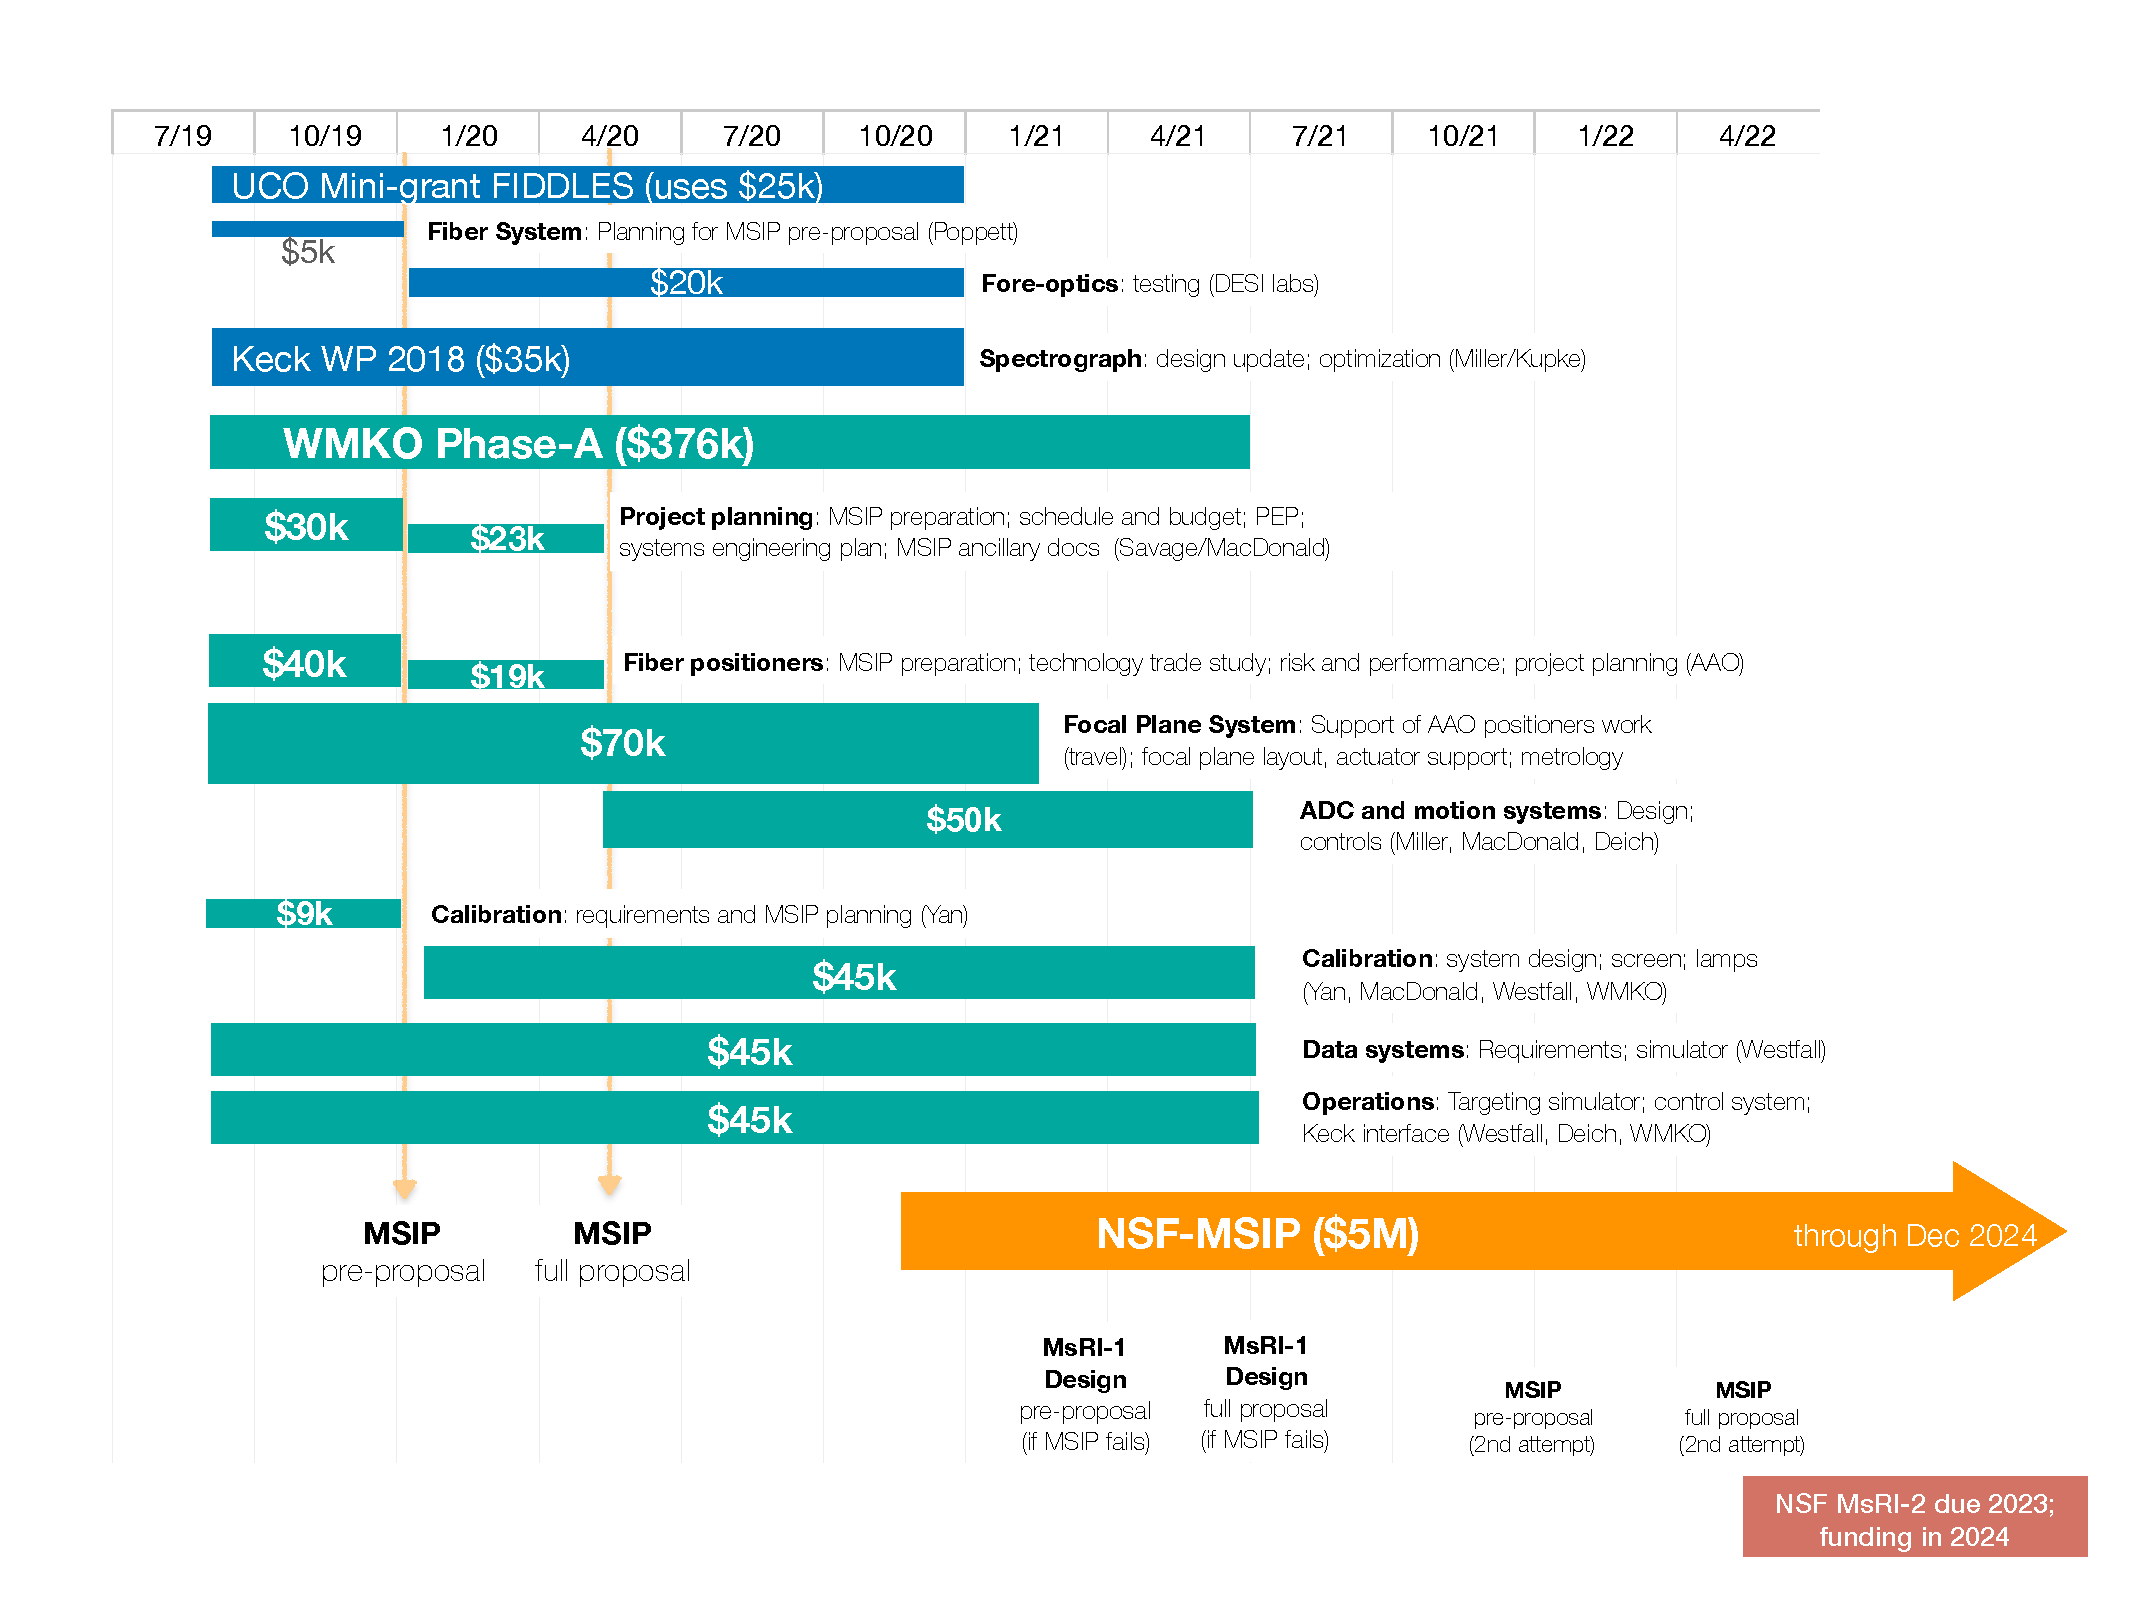
\includepdf[landscape=true]{figs/budget_schedule_schematic_v3.pdf}







\setcounter{page}{1}
\bibliographystyle{apj}
\bibliography{references}

\end{document}


